\RequirePackage[switch, columnwise, running, mathlines, displaymath,
mathlines]{lineno}
\RequirePackage{docswitch}
% \flag is set by the user, through the makefile:
%    make note
%    make apj
% etc.
\setjournal{\flag}

\documentclass[\docopts]{\docclass}

% You could also define the document class directly
%\documentclass[]{emulateapj}

% Custom commands from LSST DESC, see texmf/styles/lsstdesc_macros.sty
\usepackage{lsstdesc_macros}

\usepackage{graphicx}
\graphicspath{{./}{./figures/}}
\bibliographystyle{apj}

% Add your own macros here:
\newcommand{\textul}[1]{\underline{#1}}

\newcommand{\aim}[1]{\textcolor{red}{#1}}
\newcommand{\changes}[1]{\textcolor{blue}{#1}}

% in case I can think of some fancy formatting later\dots
\newcommand{\lsst}{\textsc{LSST}}
\newcommand{\plasticc}{\textsc{PLAsTiCC}}
\newcommand{\proclam}{\texttt{proclam}}
\newcommand{\snmachine}{\texttt{snmachine}}
\newcommand{\snphotcc}{\textsc{SNPhotCC}}

% ======================================================================

\begin{document}
\linenumbers

\title{The Photometric \textsc{LSST} Astronomical Time-series Classification Challenge (\textsc{PLAsTiCC}): Selection of a performance metric for classification probabilities balancing diverse science goals}

\maketitlepre

\begin{abstract}

  Open challenges are an effective route to promoting the development of novel techniques in astronomical data analysis.
  However, the probabilistic classifications appropriate to upcoming deep surveys, including the Large Synoptic Survey Telescope (\textsc{LSST}), are incompatible with the traditional metrics used on deterministic classifications.
  Furthermore, large survey collaborations like that of \textsc{LSST} may use the products of these challenges for diverse science objectives, indicating a need for a metric that balances a variety of goals.
  We describe the process used to develop an optimal performance metric for a challenge affected by both these issues in the context of the Photometric \textsc{LSST} Astronomical Time-series Classification Challenge (\textsc{PLAsTiCC}), an open competition aiming to identify promising methods for obtaining classification probabilities of transient and variable objects by engaging a broader community both within and outside astronomy.
  Using mock classification probability submissions exhibiting characteristic performance types anticipated of \textsc{PLAsTiCC}, we compare the sensitivity of two metrics of classification probabilities to the isolated systematics and combinations thereof, ultimately making the reassuring conclusion that multiple metrics yield qualitatively consistent results.
  Thus we choose as a metric for \textsc{PLAsTiCC} a weighted modification of the log-loss due to the availability of a meaningful interpretation and superior sensitivity to the most concerning potential failure modes.
  We propose extensions of our procedure to ever more complex challenge goals and suggest some guiding principles for approaching the choice of a metric of probabilistic classifications.

\end{abstract}

% Keywords are ignored in the LSST DESC Note style:
\dockeys{}

\maketitlepost

% ----------------------------------------------------------------------
% 

\section{Introduction}
\label{sec:intro}

The Large Synoptic Survey Telescope (\lsst) has the potential to advance time-domain astronomy, with anticipated impacts on the study of transient and variable objects (TVs) within and beyond the Galaxy.
% Bright cosmological objects like Type Ia supernova are probes of cosmological distance (and thus the expansion of the universe).
% Core-collapse supernovae encode within their stunning demise the evolution properties of massive stars.
% Bright astrophysical transients like RR Lyrae give insight into the structure and evolution of stars.
% Active galactic nuclei probe the evolution of large massive galaxies.
% These are but some of the physical principles that are testable with the many different kinds of transients that will be delivered with the Large Synoptic Survey Telescope (LSST).
With its rapid scan strategy, exquisite depth, and many photometric filters, \lsst\ will deliver millions of transient detections, enabling unprecedented population-level studies of astronomically varying sources in some cases across cosmic time.

Science from the \lsst\ dataset, however, is contingent on distinguishing classes of astrophysical sources
 from one another. The gold standard for such identification in astronomy has traditionally been
based on the spectrum of the source. However, the volume of discovered objects in the LSST, as well as their potentially high redshifts implies that the prospect of spectroscopic follow-up of a large fraction of them is difficult
with expected spectroscopic resources. Thus several science cases (such as SN cosmology) will actively depend om classification of astrophysical sources based on the photometric light curve, and possibly a much smaller training sample/model based on a spectroscopic sub-sample. 
% Using the wealth of data (for any of a multitude of science cases) requires distinguishing different classes of sources, according to the available data.
As such, there is an acute need for photometric lightcurve classifiers that can perform well on datasets data include a wide variety of sources, and where classification over the range of objects is desired, rather than challenges that focus on only one class.

Classifaction of noisy light curves is intrinsically probabilistic. Sometimes, classification can lead to identification of a category wth very high probabilities, while at other times several categories might seem approximately 
less likely. The latter is clearly the likely scenario for light curves dominated by noise.
Here, we will refer to classification schemes which preserve these probabilities as `Probabilistic Classification`.
However, often one compresses this to a  
 `Deterministic classification` which is equivalent to choosing a single category with probability 1.0 through som 
rules, obviously leading to a loss of information. The value of this loss depends on how the classification results are subsequently used. For example, when using classification of astrophysical sources to determine the use of follow-up resources, one ultimately takes a binary decision on whether to follow-up a particular source or not. While the knowlege that an object has been identified to be a particular type with an overwhelming probability (eg 0.99) is likely different to a situation where an object is simply slightly likelier to be a particular class than the remaining classes of objects is important but could be appropriately reflected in a deterministic classifier. If the follow-up resources were abundant enough to warrant the optimization of follow-up of less well classified objects,  the information in the probabilities could be useful in resource allocation. Considering the different case of supernova cosmology from a photometric classified sample of SNe, such probabilistic classifications can be propagated to subsequent analyses of cosmological parameters allowing one to extract information from the (large) part of the sample where photometric classification failed to identify a particular type with overwhelming probability \cite{roberts_zbeams:_2017}. This implies that one should plan and investigate probabilistic classification for future surveys like LSST. 
%Because of the low-signal-to-noise expected of \lsst, probabilistic classifications are more appropriate (Roberts+17) than the point estimates of previous challenges.
%Such posteriors are more valuable than point estimates, which we call deterministic classifications in this work, because of their versatility in application and encapsulation of observational and systematic error that may propagate through inference.

Classification in astronomy is often done based on images e.g.
galaxy classification \cite{2016A&C....16...34H}, supernova
classification \cite{2017ApJ...836...97C}, identifying bars in galaxies
\cite{2018MNRAS.477..894A}, separating Near Earth Asteroids from artifacts in images
\cite{2016PASJ...68..104M}, as well as light curves e.g. \cite{2016PASJ...68..104M,2017arXiv170906257M,2017CQGra..34f4003Z}, and even noise classification e.g. \textbf{check Abbot et al ref}\cite{2017CQGra..34f4003Z,2018PhRvD..97j1501G}. In most cases though, only a limited subset of types. The last such challenge viz. SNPhotCC was also restricted to a subset of classes (specifically, extragalactic explosive events).

The Photometric \lsst\ Astronomical Time-series Classification Challenge (\plasticc) aims to identify classification techniques that serve the broader astronomical community by engaging the broader community outside astronomy.
Unlike previous challenges, \plasticc\ differs in that the more comprehensive dataset includes models for well-understood classes, newly observed classes, and classes that have only been proposed to exist, to simulate serendipitous discovery anticipated of \lsst.
Additionally, \plasticc\ will join the ranks of a handful of past astronomy classification challenges hosted on \href{https://www.kaggle.com/competitions}{Kaggle}, a platform for predictive modelling, that hosts data analytics competitions where seasoned professionals and amateurs can compete to classify, model and predict large data sets uploaded by companies or scientific collaborations. It attracts a broad user base, and those without domain knowledge of astronomy may provide novel approaches to the problem of photometric classification..

A classification posterior can be propagated through population-level inference without a separate error propagation pipeline, and for the purposes of allocation of follow-up resources, a probability can always be reduced to a point estimate for the purposes of deterministic decisionmaking (such as for allocation of follow-up resources), but a deterministic classification cannot in general be used to reconstruct a probability density for an individual object.

\plasticc\ will thus accept classifiers producing classification posteriors.

However, probabilistic classifications are incompatible with the metrics of deterministic class assignments used in previous classification challenges \cite{kessler_supernova_2010, kessler_results_2010} and efforts to develop supernova classifiers \cite{2018ApJS..236....9N}.
In this context, a metric is simply a quantification of the performance of a classifier.
Notions of accuracy, purity, completeness, and other terms endemic in science are examples of traditional metrics appropriate to classification point estimates.
Many traditional classification metrics may be modified for evaluation on probabilistic classifications \cite{lochner_photometric_2016, moller_photometric_2016, hon_deep_2017, hon_detecting_2018, 2011arXiv1108.4696G} but only by reducing class probabilities to point estimates of class and evaluating those at discrete cutoffs that can affect the conclusions of the study.

If the data are simulated using a fully self-consistent forward model, a metric of the accuracy of classification probabilities relative to the true, underlying probabilities would be straightforward.
However, such a simulation procedure would require beginning with a fully populated probability space over all classes and all possible lightcurves, which is an insurmountable challenge.
Therefore, attention must be directed toward the no longer straightforward matter of defining the criterion for a winning classifier.
In the context of astronomy, concerns about the choice of metric for probabilistic classifications have been investigated only to a limited degree thus far \cite{2018SoPh..293...28F, 2017MNRAS.464.4463K}, with most approaches concentrating on the `standard' metrics of purity and completeness, however metric consistency over a range of classifiers and between different analyses is not always ensured \cite{2018A&C....23...15B}.

This work explores the two-fold problem of how to select a metric of a probabilistic data product that will be used in many science applications and thus lacks a single obvious figure of merit.

%\aim{I actually preferred the following as a list, although I agree that it could use some pruning.}
%\begin{itemize}
%\item    The metric must return a single scalar value.
%\item    The metric must be well-defined for non-binary classes.
%\item    The metric must balance diverse science use cases in the presence of heavily nonuniform class prevalence.
%\item    The metric must respect the information content of probabilistic classifications.
%\item    The metric must be able to evaluate deterministic classifications.
%\item    The metric must be interpretable, meaning it gives a more optimal value for "good" mock classifiers and a less optimal value for mock classifiers plagued by anticipated systematic errors; in other words, it must pass basic tests of intuition.
%\item    The metric must be reliable, giving consistent results for different instantiations of the same test case.
%\end{itemize}

In order for the metric to be useful in such a heterogenous challenge, we require that the metric must return a single, scalar value, while being well-defined for non-binary classes.

In addition, the metric should balance diverse science use cases in the presence of heavily non-uniform classes.
This is key given that the rates of astornomical transients of different types varies greatly: any classifier that requires a balance of types will under perform in the \plasticc\ (and other) competitions.

We impose the restriction that the metric must respenct the information content of the probabilistic classifiers.
Should a determininstic classifier (i.e. returning a ``1'' or a ``0''), that deterministic metric must be readily convertible into a probabilistic classification - and should preserve the relationships between classes accordingly.
Similarly, any probabilistic metric much be easily transferred to a deterministic one (given, e.g. given a threshold on the most likely classficiation choice).

The metric must pass basic tests of intuition,rewarding classifiers that serve our needs and penalizing those plagued by anticipated systematic errors.

And finally, the metric must be reliable, giving consistent results for different instantiations of the same test case.
While it is clear that different procedures will happen simultansously, the metric should be stable to these changes, and be able to rank different scenarious given any particular set of rules imposed upon the metric.

The Probabilistic Classification Metric (ProClaM) code used in this exploration of performance metrics is publicly available on GitHub.\footnote{\url{https://github.com/aimalz/proclam}}


\section{Data}
\label{sec:data}

We explore the behavior of the metrics on mock classifications with well-understood weaknesses as well as realistic mock classifications from past challenges.
Data is in the form of catalogs of posterior probability vectors $p(m \mid d)$ over $M$ classes $m$ conditioned on the observed lightcurve $d$, with each probability vector normalized to sum to unity.\footnote{Throughout the paper, ```data'' always refers to classification results, not lightcurves; no \plasticc\ lightcurves were simulated, viewed, or classified in the preparation of \textit{this} paper.}
% We introduce the convention that the $M^{\mathrm{th}}$ class is designated ``other'' to encompass never-before-seen classes.
\textbf{[Description of the `confusion matrix' needs fixing]} We model classifications as a confusion matrix $\mathbb{C}$, an $M\times M$ dimensional table of empirical probabilities $p(m \mid m')$ traditionally calculated from deterministic classification point estimates with knowledge of the true classes $m'$.
% TODO define TP/FP/TN/FN here and define confusion matrix in terms of them
Though probabilistic classifications are not truly compatible with the confusion matrix, we use it as a middle ground to develop intuition from conceptually familiar deterministic classifications, as has been used in astronomical contexts, \citep[e.g.][]{2012PASP..124.1175B}.

\subsection{Mock classifications}
\label{sec:mockdata}

The test cases of this section are devised to test if a metric aligns with our intuitive understanding of what constitutes a good classifier, that it should not reward classifications suffering from the most concerning failure modes, which we will refer to as \textit{systematics} throughout the paper.
We consider a data set with $M=13$ classes
% (nominally $12$ with one designated as ``other,'' meaning not represe) and
with a lognormal distribution of the number $N_{m}$ of members of each class, where $N_{m}$ spans six orders of of magnitude.

We present eight mock classifiers, each of whose efficacy is described by its confusion matrix $\mathbb{C}$.
Each classifier derives classification posteriors $p(m \mid m')$ based on the true classes as a proxy for the information contained in the lightcurves.
The posterior probability vector $p(m \mid m')$ for a given object is proportional to a perturbation of the row $\mathbb{C}_{m'}$ of the confusion matrix $\mathbb{C}$ corresponding to its true class $m'$, with a perturbation factor of $\delta=0.1$, following the Dirichlet distribution:
\begin{eqnarray}
  \label{eq:cmtoprob}
  p(m \mid m') &\propto& \Gamma{\mathbb{C}_{m'}\delta}/\sum_m'{\Gamma{\mathbb{C}_{m'}\delta}},
\end{eqnarray}

%where the perturbation vector $\vec{\epsilon}$ has components drawn from a half-Cauchy distribution
%\begin{eqnarray}
%  \label{eq:cauchy}
%  f(x) &=& \frac{2}{\delta\pi} \left(1+\left(\frac{x+x_{0}}{\delta}\right)^{2}\right)^{-1}
%\end{eqnarray}
%with $x_{0}=0$.
%Only nonnegative values can be drawn from the half-Cauchy distribution, and the constant of proportionality for Equation~\ref{eq:cmtoprob} is chosen to ensure normalization, i.e. $\sum_{m}p(m \mid m')=1$.
% \aim{[Rahul: Might be good to have a plot of the pdf when x0 takes values close to 0., something like 0.4, 0.8 and close to 1.0]}

% TODO: sequential color scheme?
% TODO: letters for panels, refer to them in text
\begin{figure*}
	\begin{center}
    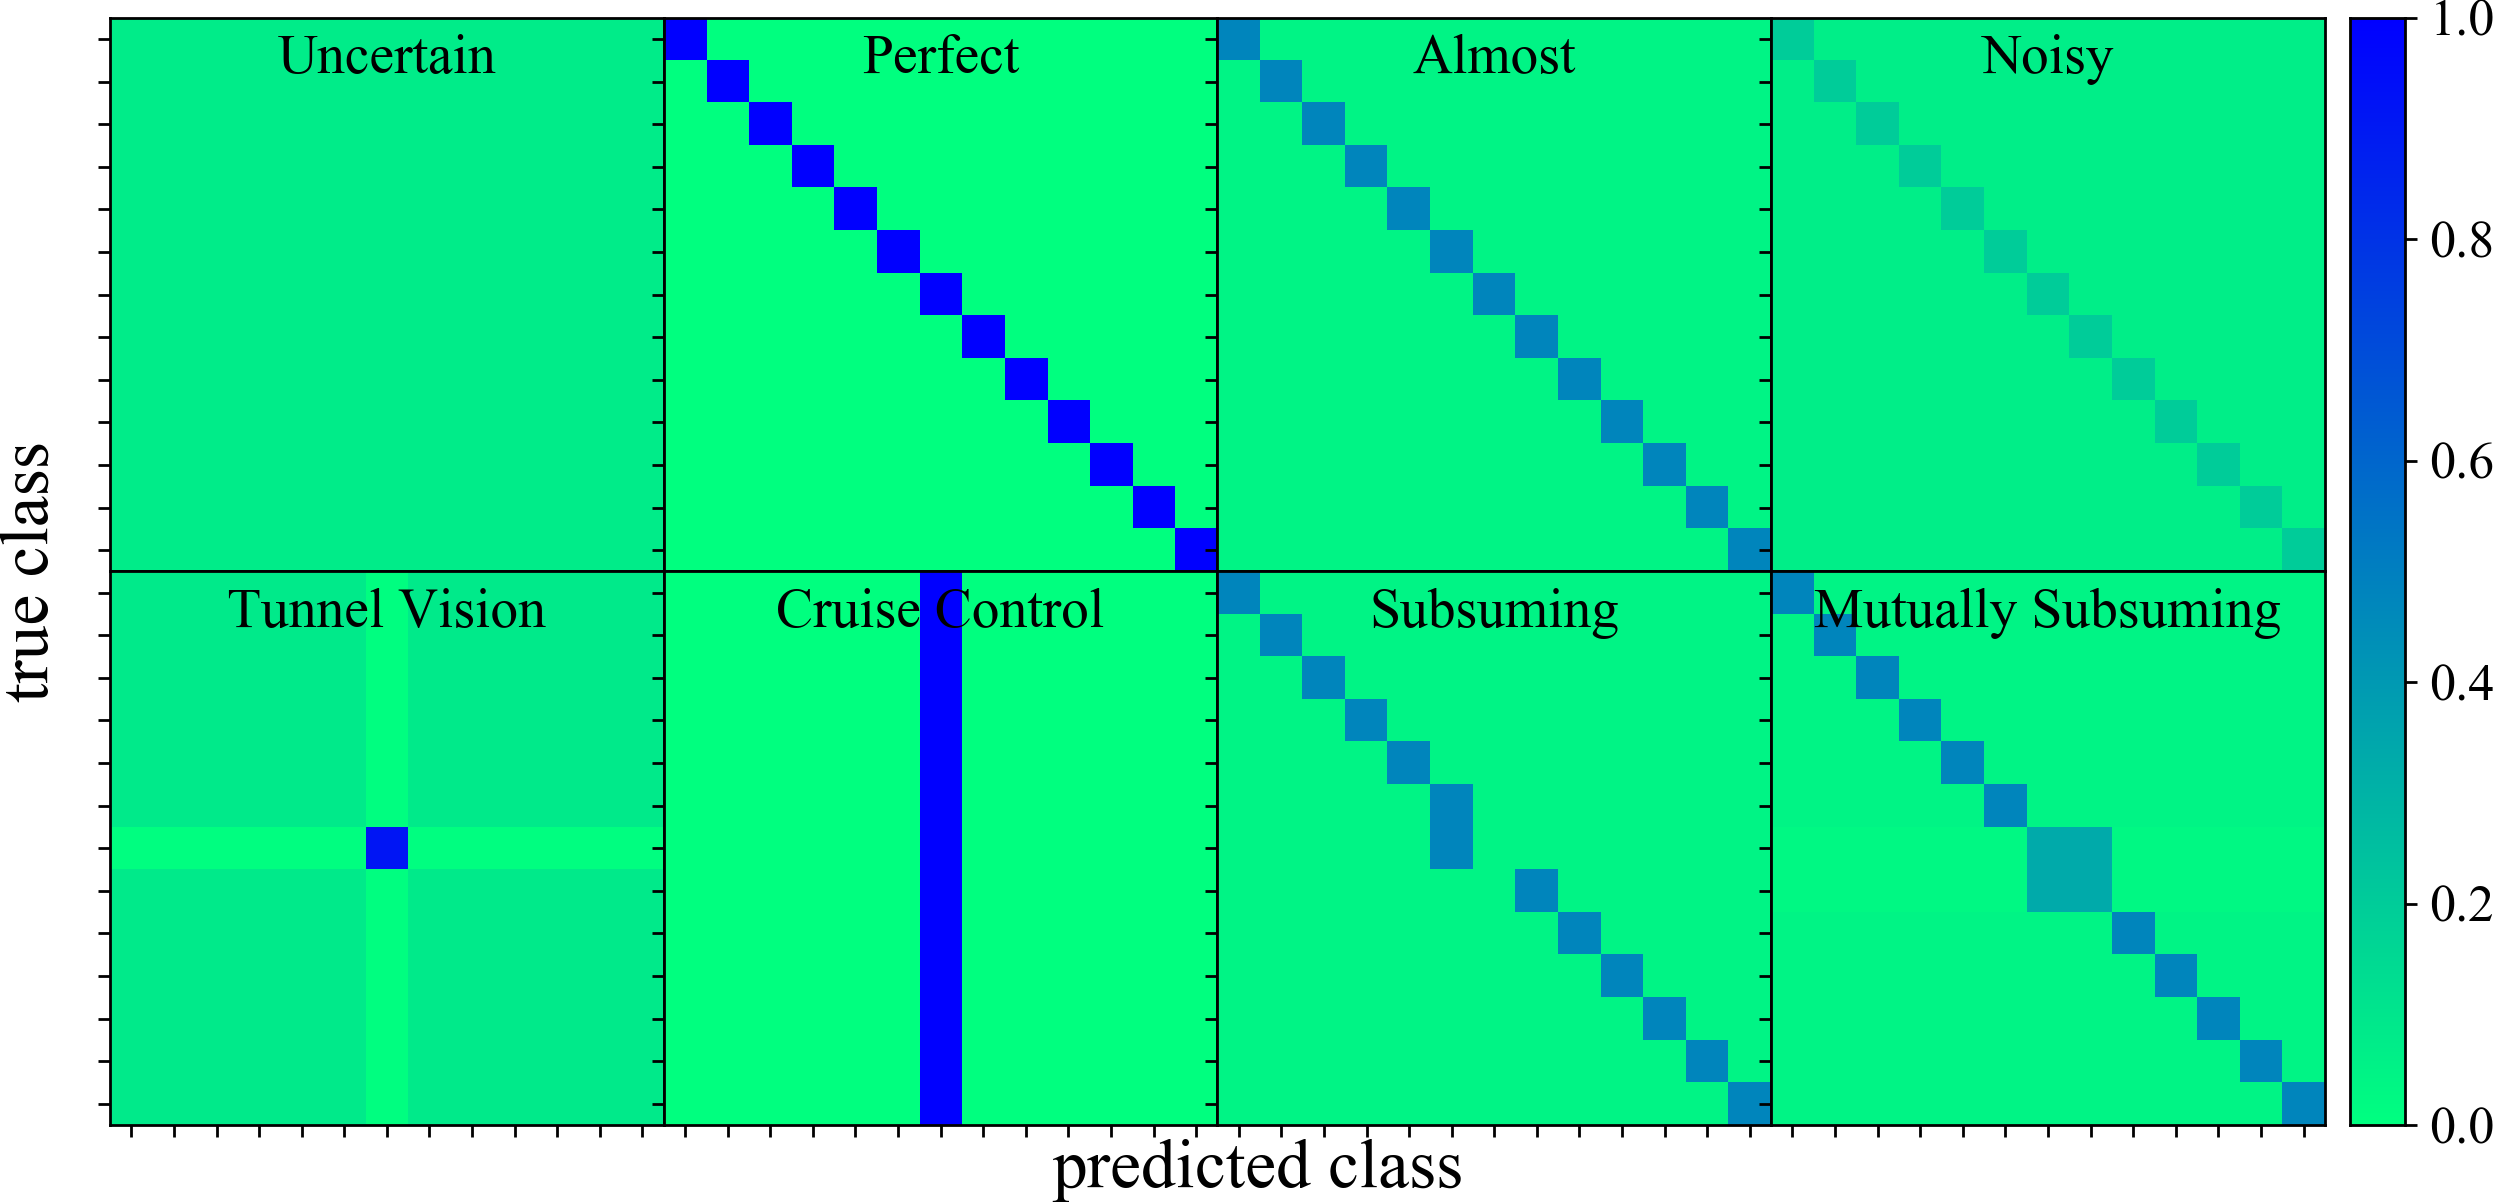
\includegraphics[width=0.8\textwidth]{./fig/all_sim_cm.png}
		\caption{Confusion matrices for eight mock classifiers.
    leftmost top: uncertain classification,
    leftmost bottom: perfect classifications,
    left-center top: almost perfect classification,
    left-center bottom: unbiased classifications,
    right-center top: perfect classification (type 1 and type 2 errors) for one class and uniform for all others,
    right-center bottom: assigning all objects the same class,
    rightmost top: consistently assign one class to another,
    rightmost bottom: consistently assign another class to one class}
		\label{fig:mock_cm}
	\end{center}
\end{figure*}

Figure~\ref{fig:mock_cm} shows the confusion matrices corresponding to each systematic considered, discussed in detail below.
For each case, we address:
\begin{enumerate}
  \item What defines this error property?
  \item Under what conditions is this error property relevant?
  \item What are our expectations of and desires for this error property's effect on metric behavior?
\end{enumerate}

\subsubsection{Uncertain classification}
\label{sec:uncertaindata}

An entirely uniform confusion matrix $\mathbb{U}$ (leftmost top panel of Figure~\ref{fig:mock_cm}) would correspond to uniform random guesses for deterministic classification, but the probability vectors drawn from it are more nuanced.
In accordance with Equation~\ref{eq:cmtoprob}, the probability vectors are perturbations away from a uniform distribution across all classes.
The peak values of these probability vectors will correspond to uniform random classifications, however, with $p(m' \mid d)\approx M^{-1}$.
We can consider the \textit{uncertain} classifier as an experimental control for the worst possible classifier, bearing in mind that if classifications were anticorrelated with true classes (i.e. consistently misclassifying A as B and B as A), the experimenter would simply reassign the classification labels to improve performance.

\subsubsection{Accurate classification}
\label{sec:accuratedata}

The \textit{perfect} classifier has a diagonal confusion matrix $\mathbb{I}$ (leftmost bottom panel of Figure~\ref{fig:mock_cm}), which would correspond to deterministic classifications that are always correct.
In terms of probabilistic classifications, a perfect result would be a probability vector with 1 for the true class and 0 for all other classes.
Due to our addition of the random perturbation factor $\vec{e}$, the probability vectors drawn from the perfectly diagonal confusion matrix are randomly perturbed away from perfect classifications by the small factor $\delta$, but the class with maximum probability is almost always still the true class, to the tune of $\sim0.96$ with our choice of $\delta$.
This case is also a control, in that \plasticc\ would not be necessary if we believed the perfect classifier were realistically achievable.

In addition to a perfect classifier, we test linear combinations
\begin{eqnarray}
  \label{eq:lincomb}
  \mathbb{C}^{\mathrm{acc}; s} &=& \frac{1}{M+s-1} \left(s\mathbb{I} + \mathbb{U}\right)
\end{eqnarray}
of the perfect and uncertain classifier confusion matrices where the contribution of the perfect classifier is greater than that of the uncertain classifier by a factor of $s$.
Deterministic classifications drawn from such a confusion matrix would be correct $s$ times as often as they are wrong, and the incorrect guesses would be uncorrelated across classes.
The probability vectors drawn from such confusion matrices would have some variability but still mostly have their peak value at the truth.
We consider the case of the \textit{almost perfect} classifier with $s=4$ (left-center top panel of Figure~\ref{fig:mock_cm}) and the \textit{noisy} classifier with $s=2$ (left-center bottom panel of Figure~\ref{fig:mock_cm}), which correspond to $p(m' \mid d)\approx0.82$ and $p(m' \mid d)\approx0.62$ respectively.
We expect that the response to variation in $s$ may differ across metrics.
(Though $s$ would realistically be expected to vary for each class, we do not conduct a systematic investigation of this possibility at this time.)

A classifier with different accuracy for each class may be considered a systematic in its own right.
An extreme example of such a classifier could be one with perfect classification performance on one class and uncertain classification on all others; its confusion matrix would be uniform except for one row, which would take a value of unity on the diagonal and zero elsewhere.
Such a classifier would have high value to those who study the class with perfect performance and should still be used in the context of \lsst.
For the purposes of \plasticc, we take a more measured approach, and require that the \plasticc\ metric must serve the needs of those who study a wide variety of classes for different purposes. Hence, from the perspective of \plasticc, such a \textit{tunnel vision} classifier (right-center panel of Figure~\ref{fig:mock_cm}) is a major concern.
%However favoritism is inappropriate for the overall \plasticc\ metric, which must serve the needs of those who study all the classes and for different purposes.
\subsection{Inaccurate classification}
\label{sec:inaccuratedata}

Inaccurate classification in the context of a deterministic classifier is self-explanatory.
If a classifier is \textit{systematically} inaccurate, its confusion matrix has significant probability on off-diagonal elements.
We model inaccurate probabilistic classifications of class $m'$ by using the row of the confusion matrix corresponding to class $\tilde{m}$ as the basis for the perturbed probability vector
\begin{eqnarray}
  \label{eq:subsume}
  p(m\ \mid\ m') = p(m\ \mid\ \tilde{m}).
\end{eqnarray}
Class $m'$ is said to be \textit{subsumed} by class $\tilde{m}$ for such a classifier.
The asymmetric relationship between $m'$ and $\tilde{m}$ is illustrated in the rightmost top and bottom panels of Figure~\ref{fig:mock_cm} for class $m'$ being subsumed by class $m'-1$ and class $m'$ subsuming class $m'+1$, respectively.

Subsuming is particularly expected when distinguishing between subtypes of some class, and it is of utmost importance when the subtypes have wholly different science applications.
Classification subtypes that are useful for completely different science cases are found in supernova classification, through e.g. the differences between SN Ia and SN Ibc. SN Ia and SN Ibc are challenging to distinguish, and the former often subsumes the latter in common classifiers, an effect that can be exacerbated by underrepresentation of SN Ibc in available training sets.
However, using SN Ibc in the traditional cosmology analysis done with SN Ia can bias estimates of the cosmological parameters, so the distinction is critical. 

Similarly RRc and RRd Lyrae stars have different pulsation modes (RRc stars pulsate in the first overtone, while RRd stars pulsate simultaneously in the fundamental mode and first overtone, and are much more rare than RRc stars), and yet are challenging to separate observationally. We would like the \plasticc\ metric to identify the strength of a classifier that successfully prevents this kind of error.

An extreme case of inaccurate classification is to classify all objects as the most common class, a particular concern for \plasticc\ given the potential for population imbalance between classes.
For our purposes, it matters not whether the subsuming class is actually the most common or only the most common in the training set.
Such a \textit{cruise control} classifier (right-center bottom panel of Figure~\ref{fig:mock_cm}) counters \plasticc's goal of identifying objects belonging to extremely rare classes, particularly if the metric weights all objects equally.
Though we dampen this systematic by employing per-class weights, described in Section~\ref{sec:weights}, we nonetheless examine its impact under other plausible weighting schemes.

% \subsubsection{Combination of systematics}
% \label{sec:combo}
%
% \begin{figure}
% 	\begin{center}
% 		% 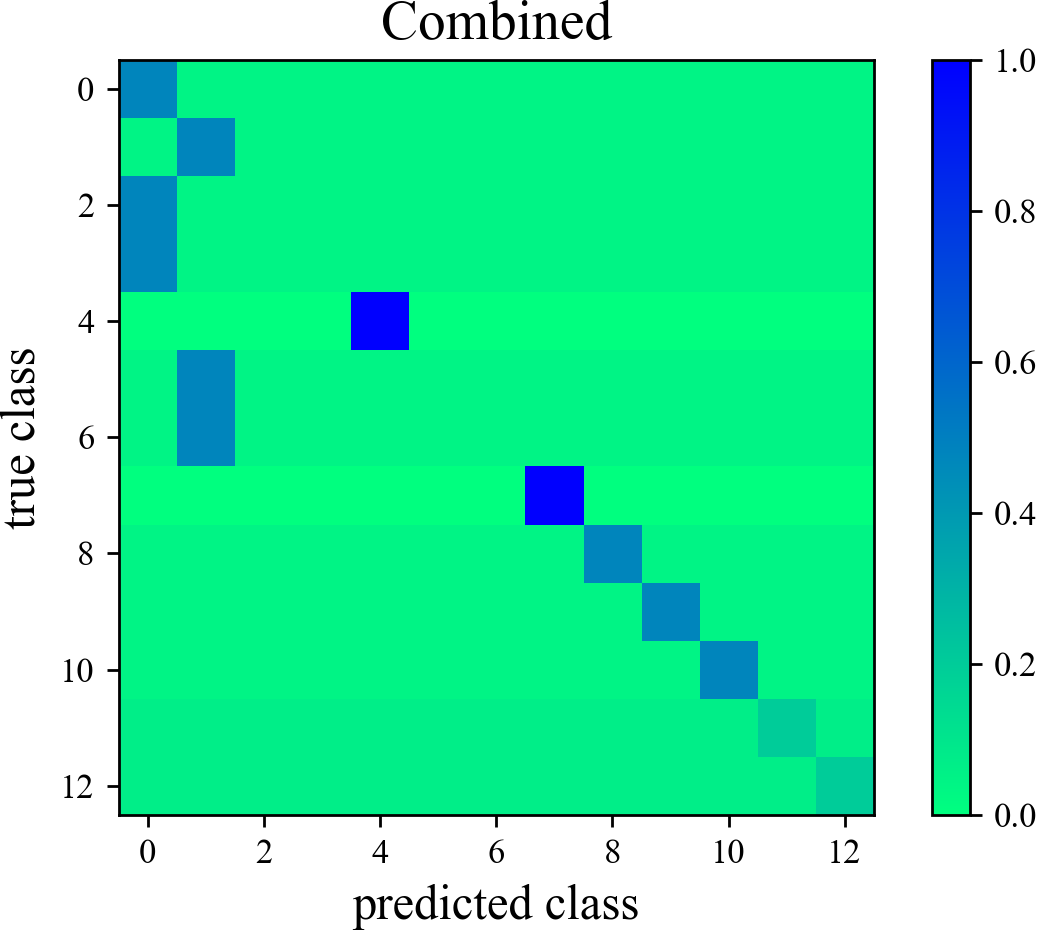
\includegraphics[width=0.45\textwidth]{./fig/Combined.png}
% 		\caption{}
% 		\label{fig:combo_cm}
% 	\end{center}
% \end{figure}

\subsection{Representative classifications}
\label{sec:realdata}
%\aim{This would be more meaningful if we were given the confusion matrices of actual submissions to \snphotcc\ and then checked whether the \plasticc\ metric would have designated a different winner.
%Also, it may be more interpretable if we instead use Ashish's confusion matrices that have more classes.}

In addition to our mock classifiers, we test our metric candidates on realistic classification results unrelated to \plasticc.
The Supernova Photometric Classification Challenge (\snphotcc) \citep{kessler_supernova_2010} focused on classifying the lightcurves of a heterogenous population into a limited number of subclasses, with a goal of identifying one particular type of object for a single scientific application.
The \snphotcc\ attracted diverse classification approaches, including $\chi^{2}$ fits of the supernova lightcurves to publicly available templates \citep{2002PASP..114..803N} physical models \citep{2008ApJ...681..482C}, and empirical models, as well as alternatives to curve-fitting such as
%, and a linear slope to magnitudes per day was used for the non-Ia sample.
outier identification on the training set Hubble diagram, dimensionality reduction,
% TODO cite InCA?
and clustering.
% A general light curve shape (rather than one motivated by the physical differences between SNeIa and core collapse SNe) was assumed by some competitors and then a kernel density estimation was performed over the fit parameters, with various approaches employed including boosting over the feature space.
Machine learning was also employed, using features such as the light-curve slopes to produce a predictive model for the training data.
% TODO need citations of ML submissions to SNPhotCC
In short, \snphotcc\ attracted physically motivated template-based methods sensitive to the differences between the test data and the template set
%, which are prone to bias given non-representativity of the test data and agnostic
as well as those based on decomposition of the light curves into generic features at risk of neglecting available physical information.

After the \snphotcc\ concluded, the lightcurves became a testbed for a suite of machine learning classifiers.
We consider one such compilation of methods, as presented in \citet{lochner_photometric_2016}, whose confusion matrices are shown in Figure~\ref{fig:snphotcc_cm}.
% TODO what are the 3 classes?
These classification algorithms include a wavelet decomposition of the spectra to construct the features over which to classify (\citet{2011MNRAS.414.1987N}, bottom row) and template-based classification procedures (\citet{2011ApJ...738..162S}, top row), each paired with Boosted Random Forest, K-Nearest Neighbors, Naive Bayes, Support Vector Machine, and Neural Network machine learning algorithms (columns).
While the complexity of entries to the \snphotcc\ was greater than this subset, we use these illustrative examples as a useful comparison set over which to assess the performance of the approaches under our metric scheme.

\begin{figure*}
	\begin{center}
    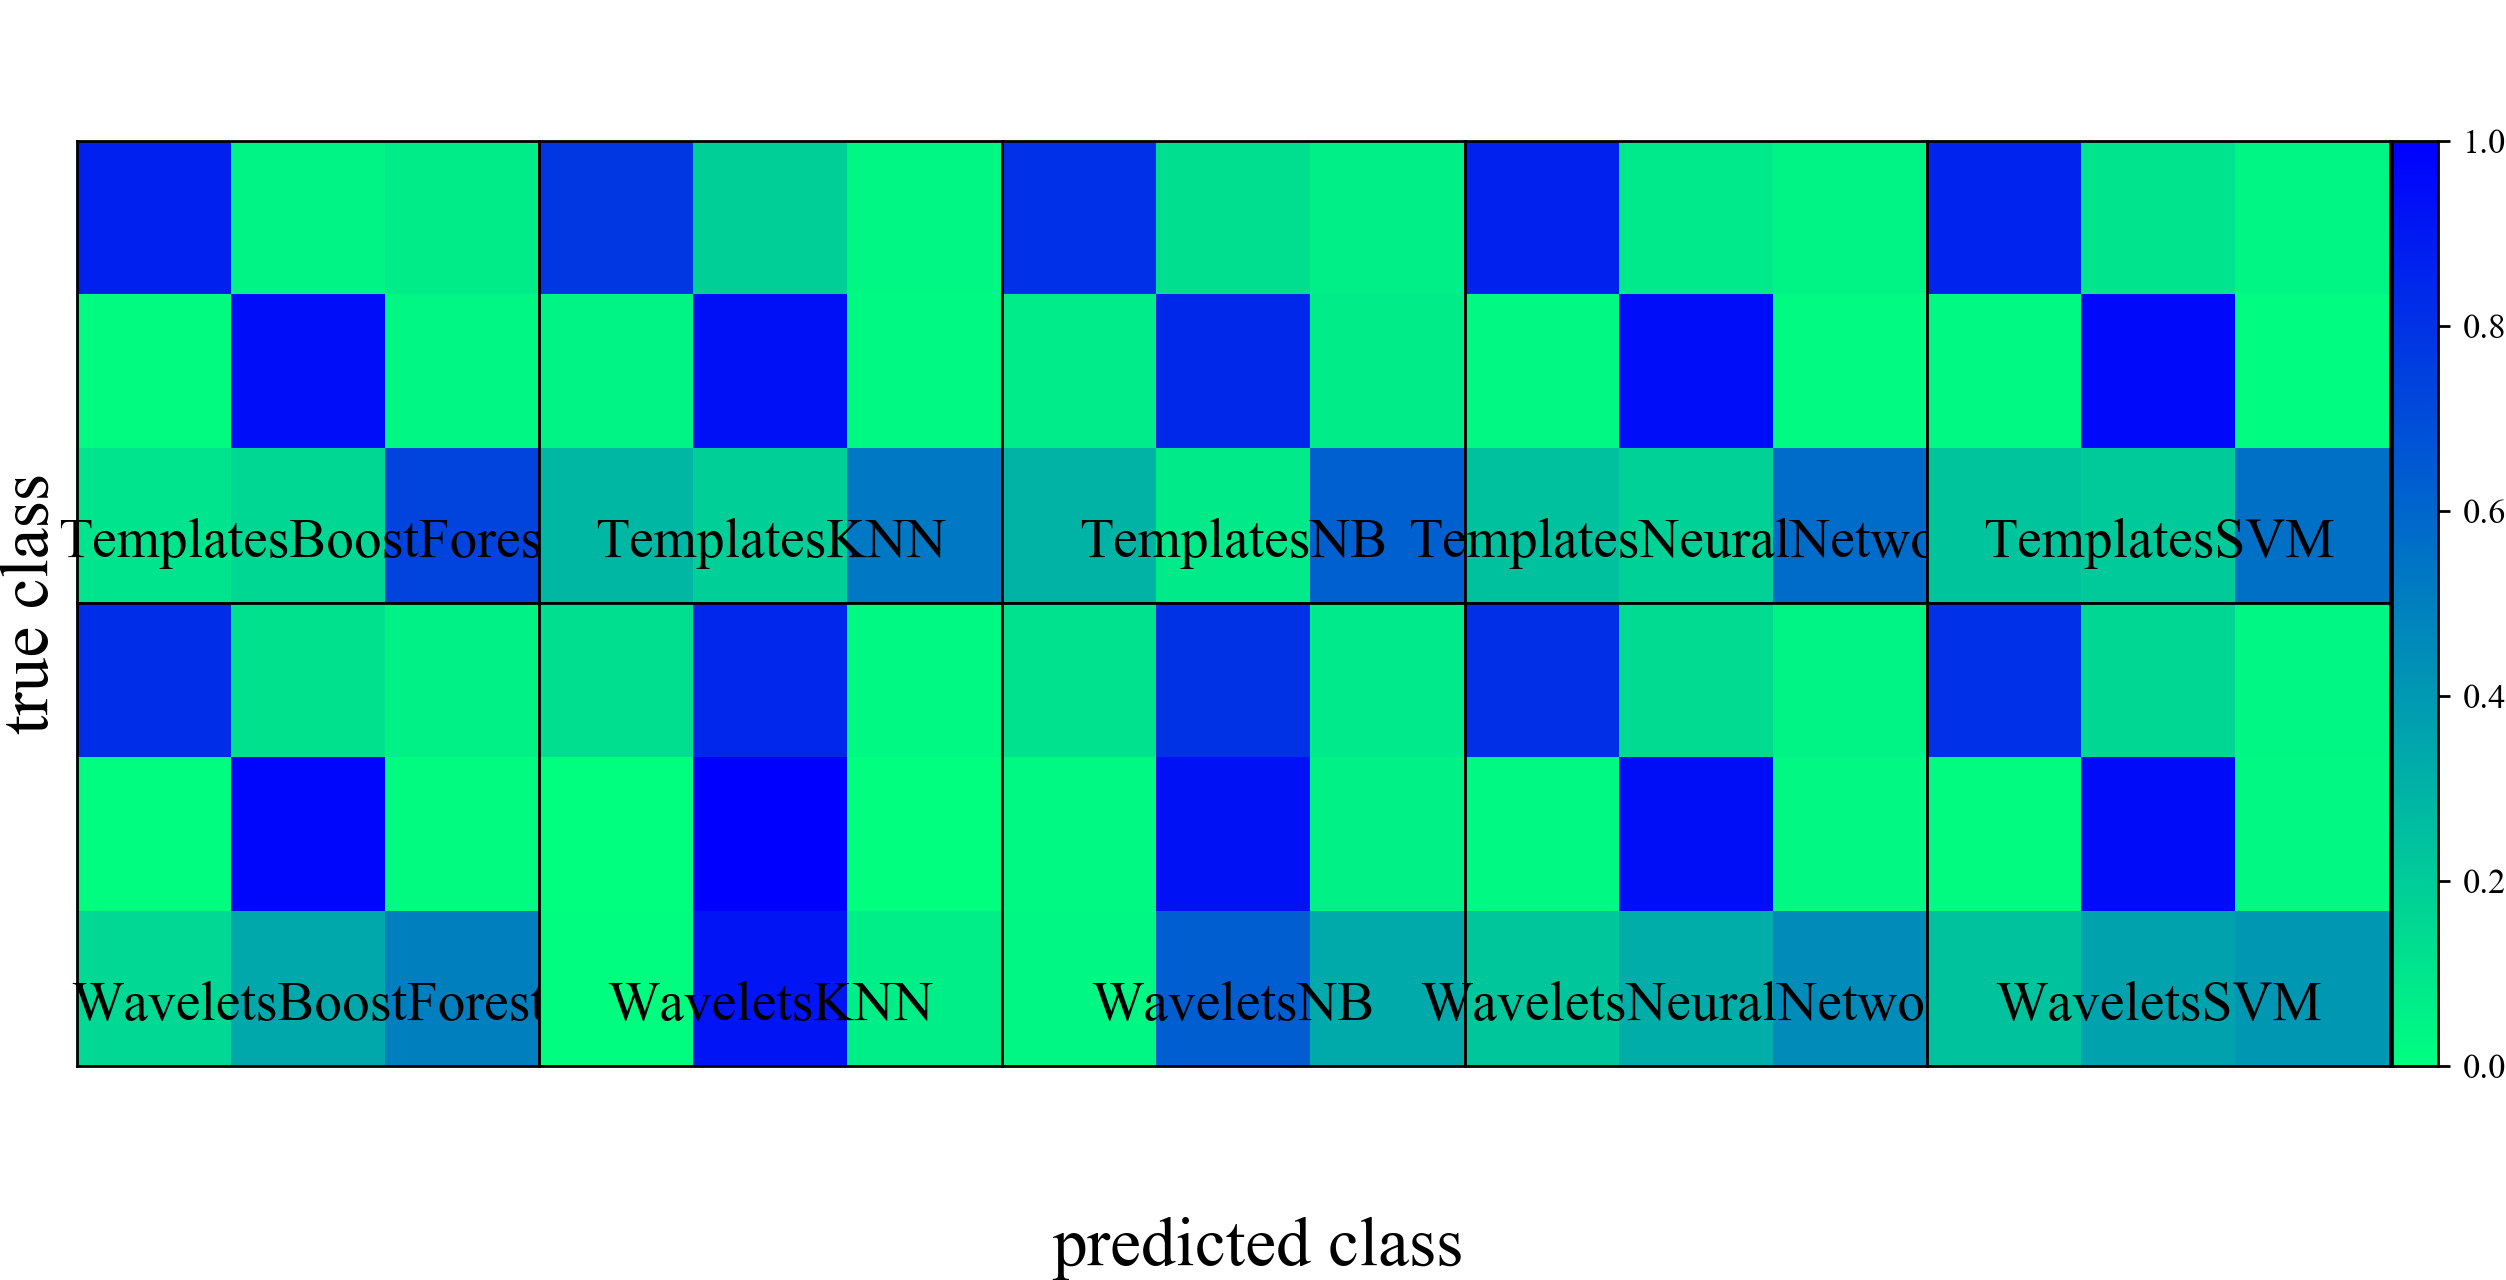
\includegraphics[width=\textwidth]{./fig/all_snphotcc_cm.png}
		\caption{Confusion matrices of the \citet{lochner_photometric_2016} methods applied to the \snphotcc\ dataset.
    Top row: five machine learning methods applied to template decompositions.
    Bottom row: the same five machine learning methods applied to wavelet features.}
		\label{fig:snphotcc_cm}
	\end{center}
\end{figure*}

We draw attention to the presence of the systematics introduced in Section~\ref{sec:mockdata} in these realistic classification results.
Note that the ``WaveletsNN'' and ``WaveletsNB'' methods both suffer from the cruise control systematic.
Nearly all the others exhibit classifications that are almost perfect for the first class, perfect for the second class, and noisy for the third.

% \subsubsection{Unknown dataset}
% \label{sec:mystery}
%
% \begin{figure*}
% 	\begin{center}
% 		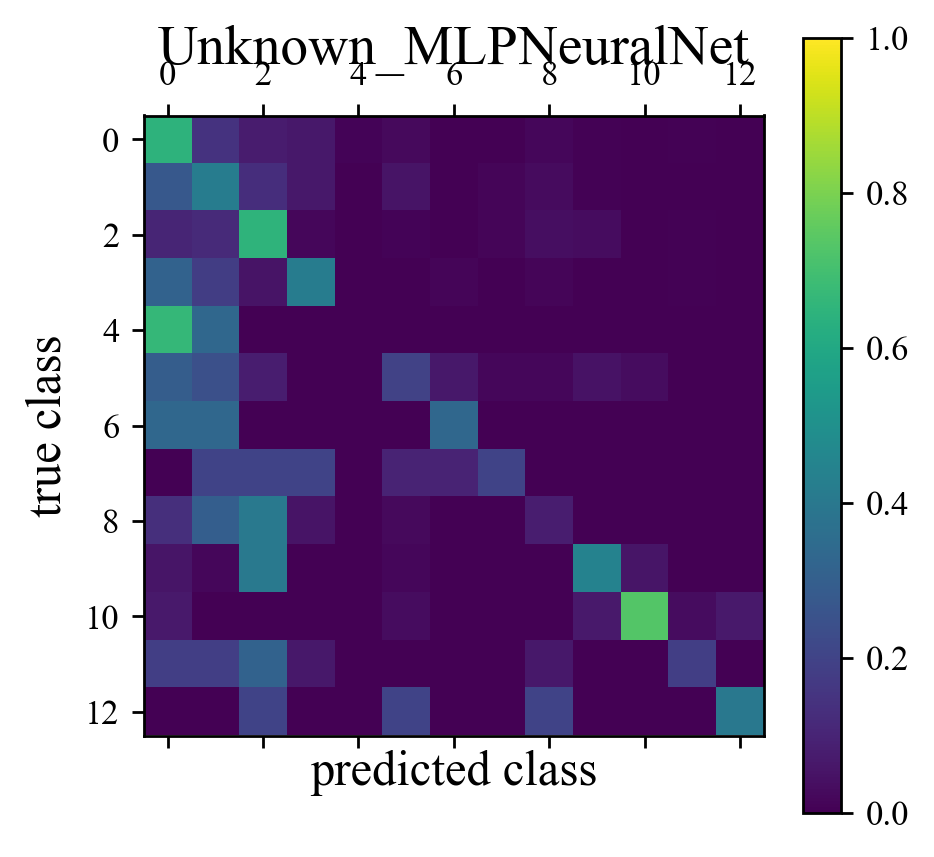
\includegraphics[width=0.3\textwidth]{./fig/Unknown_MLPNeuralNet_cm.png}
% 		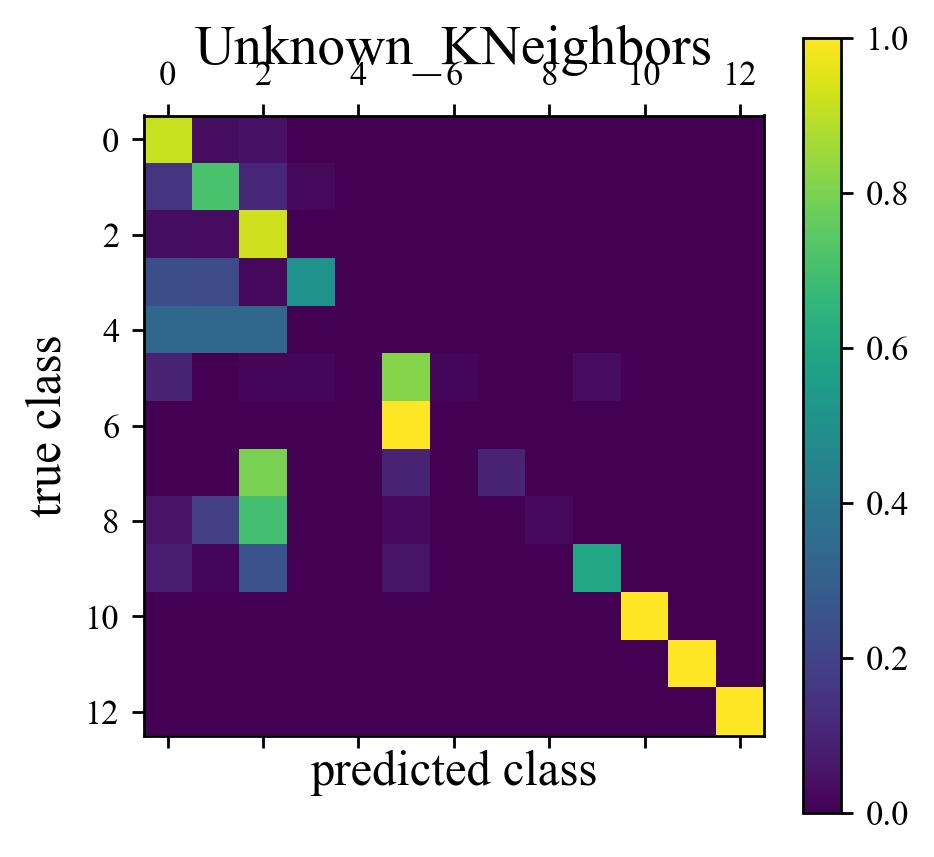
\includegraphics[width=0.3\textwidth]{./fig/Unknown_KNeighbors_cm.png}
% 		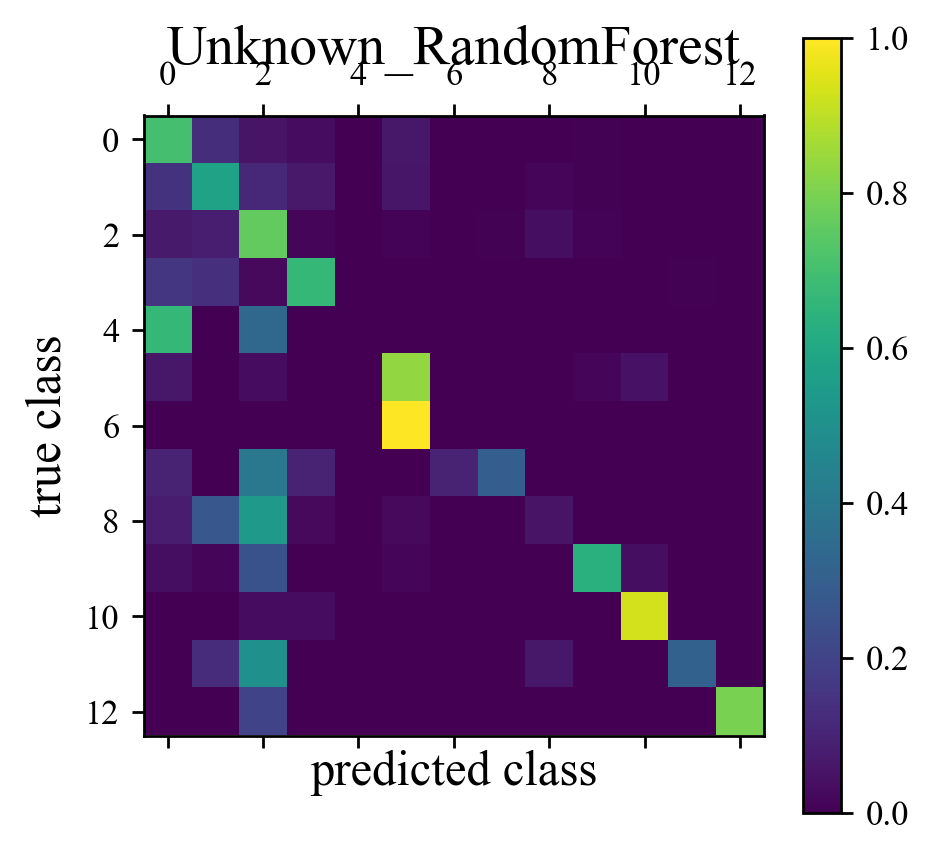
\includegraphics[width=0.3\textwidth]{./fig/Unknown_RandomForest_cm.png}
% 		\caption{}
% 		\label{fig:unknown_cm}
% 	\end{center}
% \end{figure*}


\section{Methods}
\label{sec:methods}

%\begin{itemize}
%\item    The metric must return a single scalar value.
%\item    The metric must be well-defined for non-binary classes.
%\item    The metric must balance diverse science use cases in the presence of heavily nonuniform class prevalence.
%\item    The metric must respect the information content of probabilistic classifications.
%\item    The metric must be able to evaluate deterministic classifications.
%\item    The metric must be interpretable, meaning it gives a more optimal value for "good" mock classifiers and a less optimal value for mock classifiers plagued by anticipated systematic errors; in other words, it must pass basic tests of intuition.
%\item    The metric must be reliable, giving consistent results for different instantiations of the same test case.
%\end{itemize}

To optimally discriminate between classification techniques, there must be a performance metric, a single scalar value quantifying how appropriate a classifier is for the task at hand.
Choosing a metric for \plasticc\ therefore is logically entwined with the challenge goals.
The goal of \snphotcc\ was to identify good classifiers of SN Ia used for a photometric cosmology analysis, which lends itself to a metric that optimizes the purity of any resultant data set.
\plasticc, on the other hand, differs from \snphotcc\ in that its goals are not tied to one application or even one type of T\&V class.
As such, the choice of a metric is not so simple for \plasticc's diverse science goals.

%he posterior probabilities of class must be accurate for use in inference, and they must be evaluated in a way that does not excessively favor any one science application.

In Section~\ref{sec:deterministic}, we review familiar classification metrics in astronomy.
In Section~\ref{sec:probabilistic}, we introduce metrics appropriate for probabilistic classification.
We take weighted averages of the per-object metrics with per-class weights described in Section~\ref{sec:weights}.

\subsection{Deterministic metrics}
\label{sec:deterministic}

We begin with a presentation of a subset of classification metrics that have been used in the evaluation of astronomical lightcurve classifiers in the recent past.
The metrics we highlight make use of the notions of true positive, false positive, and false negative counts from binary deterministic classification.
We briefly define the \textit{efficiency} $\epsilon \equiv \mathrm{TP} / (\mathrm{TP} + \mathrm{FN})$ and \textit{purity} $\pi \equiv \mathrm{TP} / (\mathrm{TP} + \mathrm{FP})$.

\subsubsection{Science-motivated metrics}
\label{sec:science}

As the \snphotcc\ was only concerned with SN Ia cosmology, it was effectively binary, in that the metric did not distinguish between non-Ia classes.
The \snphotcc\ metric $\mathcal{FOM} \equiv \epsilon \cdot \tilde{\pi}$,
% \begin{eqnarray}
%   \label{eq:snphotccfom}
%   \mathcal{FOM} &\equiv& \epsilon \times \tilde{\pi}
% \end{eqnarray}
is the product of the efficiency
% \begin{eqnarray}
%   \label{eq:efficiency}
%   \epsilon_{Ia} &=& \frac{N_{Ia}^{\mathrm{true}}}{N_{Ia}^{TOT}}
% \end{eqnarray}
of SN Ia classification and a modification $\tilde{\pi} \equiv \mathrm{TP} / (\mathrm{TP} + r \mathrm{FP})$ of the purity in terms of a penalty factor $r$
% \begin{eqnarray}
%   \label{eq:pseudopurity}
%   \tilde{P}_{Ia} &=& \frac{N_{Ia}^{\mathrm{true}}}{N_{Ia}^\mathrm{true} + W_{Ia}^\mathrm{false}N_{Ia}^\mathrm{false}}
% \end{eqnarray}
% with an additive penalty term with weight $W_{Ia}^\mathrm{false}$
motivated by the potential impact on cosmological parameter constraints due to contamination of the SN Ia sample by non-Ia classes.
The pseudo-purity can be interpreted as the traditional purity when $r = 1$.
The \snphotcc\ chose $r = 3$ based on a conservative limit on the acceptable amount of spectroscopic follow-up resources to waste on non-Ia targets.
% on was related to the size of the spectroscopic subsample as roughly $w = 1 + \epsilon_{spec}^{-1} \gg 1$ but the conservative limit of $W_{Ia}^\mathrm{false} = 3$ was chosen.
% to penalize wasted spectroscopic time over rejected SNe.

% \subsection{Modified deterministic metrics}
% \label{sec:auc}

% \aim{TODO: write about AUC so it can be included in results since Michelle calculated it for us!}
% While commonly-used metrics like Receiver Operator Characteristic (ROC) curve (which maps the true positive rate against the false positive rate) and the area under the curve (AUC) can be used to infer probabilities from such classifiers, the fact that \plasticc\ is by construction simulating multiple types of objects makes the extension of ROC as a metric infeasible.

\subsection{Probabilistic metrics}
\label{sec:probabilistic}

In contrast to \snphotcc's single goal of optimal deterministic classification of a single class, \plasticc\ seeks to identify classifiers that produce classification posteriors.
We consider two metrics of classification probabilities that avoid reducing probabilities to deterministic labels.
These metrics are somewhat more involved than those of Section~\ref{sec:deterministic}, requiring additional infrastructure.

% \aim{TODO: will need to fix indexing at 0 in plots!}
Our probabilistic metrics are composed of quantities defined for each possible class $m$ available to lightcurve $n$, which is a true member of the set $\mathbb{S}_{m'}$ of astrophysical sources of class $m'$.
The metric value $Q_{n} = \sum_{m=1}^{M} Q_{n, m}$ for a single lightcurve $n$ is a sum of the per-class per-lightcurve metric values $Q_{n, m}$.
The metric value $Q_{m'} = \sum_{n \in \mathbb{S}_{m'}} Q_{n}$ for an entire class $m'$ is the sum of the per-lightcurve metrics.
Section~\ref{sec:weights} discusses how the global metrics are derived from the per-class metrics $Q_{m'}$.
As part of the derivation of the per-class per-lightcurve metrics, we also define the indicator variable
\begin{eqnarray}
  \label{eq:indicator}
  \tau_{n, m} &\equiv& \begin{cases}
  0 & m' \neq m\\
  1 & m' = m
  \end{cases}.
\end{eqnarray}

\subsubsection{Log-loss}
\label{sec:logloss}

The log-loss is a quantity borrowed from information theory and is related to a notion of \textit{entropy} $H_{n} = - \sum_{m=1}^{M} p(m \mid d_{n}) \ln[p(m \mid d_{n})]$, a measure of the space of possible states a system can have, which is in this case the class of which a lightcurve can be a member.
A classification posterior $p(m \mid d_{n})$ has minimal entropy if it takes a value of $1$ at some class and values of $0$ at all others, i.e. if it can trivially be reduced to a deterministic classification, because this is the scenario in which there is only one possible state, that the lightcurve has a true class $m$.
This definition of entropy, however, is a property of the probability $p(m \mid d_{n})$ and has no relation with any concept of the true class of the lightcurve $m'$.

To reconcile the classification posterior with the true class known by those running a challenge, we define the cross-entropy
\begin{eqnarray}
  \label{eq:logloss}
  L_{n} &=& -\sum_{m=1}^{M} \tau_{n, m} \ln[p(m \mid d_{n})],
\end{eqnarray}
which can be interpreted as the spuriously oversized space of possible states (an increase in disorder) due to using the classification posterior in place of the indicator variable.
Whereas $H_{n}$ is minimized to a value of $0$ by any deterministic classification, $L_{n}$ is minimized to a value of $0$ only if $\tau_{n}$ and $p(m \mid d_{n})$ are equal to one another.
It can also be proven that the uncertain classifier of Section~\ref{sec:uncertaindata} maximizes $L_{n}$ \citep{murphy_machine_2012}.
As an aside, a difference between $L_{n}$ and $H_{n}$ evaluated at $\tau_{n, m}$ would be the information lost to disorder in using $p(m \mid d_{n})$ in place of $\tau_{n, m}$, also known as the Kullback-Leibler Divergence (KLD); see \citet{malz_approximating_2018} for a comprehensive exploration of the KLD for a continuous 1-dimensional probability space.

The log-loss has only recently established a presence in the astronomy literature \citep{hon_deep_2017, hon_deep_2018}.
Its greatest strength is that it is straightforwardly interpretable, enabling the metric itself to directly contribute to uncertainty propagation in an inference problem using the probability densities provided by the classifier.
% \aim{[Rahul: Are you saying you could rewrite a BEAMs like model in terms of the logloss metric rather than the Probabilities P(m|d)?]}
% \aim{[Alex: Not rather than, but as the performance metric of how it's doing.  When propagated through a cosmology calculation, we'd be able to say that BEAMS improves the cosmological parameters by preserving X more information than the alternative.]}

\subsubsection{Brier score}
\label{sec:brier}

The Brier score \citep{brier_verification_1950}, given as
\begin{eqnarray}
  \label{eq:brier}
  B_{n} &=& \sum_{m=1}^{M} (\tau_{n, m} - p(m \mid d_{n}))^{2},
\end{eqnarray}
is a mean square error calculated between the indicator variable and the classification posterior.
Unlike the log-loss, the Brier score has been used extensively in solar flare forecasting \citep{crown_validation_2012, mays_ensemble_2015, florios_forecasting_2018}, stellar variability identification \citep{richards_construction_2012, armstrong_k2_2016}, and star-galaxy separation \citep{kim_hybrid_2015}.

As with the log-loss, the Brier score is minimized to $0$ only for a perfect classifier.
The Brier score is an attractive option because it both rewards classifiers for  assigning more probability to the true class and penalizes classifiers for assigning any probability to classes other than the true class, in contrast to the log-loss, which only explicitly accounts for probability assigned to the true class.
We expect this difference to significantly distinguish the Brier score from the log-loss.

The interpretation of the Brier score is less obvious than that of the log-loss, as its dimensions depend on those of the probability space upon which the classification posteriors are defined.
In addition, modifying it with weights requires choosing whether to weight only per-object values $B_{n}$ or also the individual terms $B_{n, m}$ contributing to it.
We leave to future work the thorough investigation of a nontrivial weighting scheme on the Brier metric, however, opting to treat both metrics the same, according to the weighting scheme of Section~\ref{sec:weights}, in our implementation.

\subsection{Weights}
\label{sec:weights}
% TODO: motivate weights as opposed to flat
% TODO: rename section

The most concerning systematics discussed in Section~\ref{sec:mockdata} are those of tunnel vision and cruise control.
The actual lightcurve data stream of \lsst\ will be particularly vulnerable to both due to extreme class imbalance and hierarchy punctuated by nonrepresentative training data, so \plasticc\ must include all these effects.
Any metric under equal weight per lightcurve would incentivize tunnel vision and cruise control focused on the most prevalent class.
In order to meet the needs of science cases concerning other, rarer classes, \plasticc's metric will obviously have to be more nuanced, even if it complicates the interpretability of the metric.
% This can be problematic because our science needs might require accurate classifications of uncommon classes as well.
% Because tunnel vision is actually strong performance, it is common for tunnel classifiers to dominate challenges.
% Under a ``winner takes all'' challenge and with equal weight per lightcurve, \plasticc\ would be particularly vulnerable to a tunnel vision classifier winning despite not meeting the needs of those studying less common classes.

One option is to apply a threshold of classification efficacy on all classes in order to assign an overall winner, though it would require reducing the classification probabilities to deterministic class labels.
When doing binary classification with a method that reduces probabilities to deterministic class labels, each lightcurve is assigned the class of higher probability, even if the two probabilities are quite similar, a situation that is particularly likely if the lightcurve, in fact, belongs to a third class or if the two classes are subclasses of a single physical phenomenon.
%We thus anticipate it to be a more severe issue for \plasticc\ and other realistic multi-class challenges as well as any challenges with multiple subclasses.
A simple reduction to a deterministic label could be made more palatable with a secondary threshold mechanism.
For example, requiring a minimum difference in probability density between the maximum probability class and the next highest probability class would help avert this degeneracy.
% (e.g. a newly discovered supernova with a very small number of points may be indistinguishable from a Cataclysmic variable going through a brightening).

A simpler alternative that we systematically investigate in this paper is to use a weighted average
\begin{eqnarray}
  \label{eq:weightavg}
  Q &=& \frac{1}{\sum_{m} w_{m}} \sum_{m=1}^{M} w_{m} Q_{m}
\end{eqnarray}
of per-class metrics.
Weights that are not proportional to the number of true class members and are not equal to $M^{-1}$ may be chosen to encourage challenge participants to direct more attention to classes with less active classification efforts or those that have been historically more difficult to classify due to observational limitations.

Downweighting the metrics of classes affected by counterproductive systematics could mitigate the impact of the tunnel vision or cruise control classifiers.
The weights for the \plasticc\ metric, however, must be determined before there is knowledge of which systematics affect which classes.
Because of this, the choice of weights is isolated to an inherently human problem dictated by the value placed on the scientific merits of knowledge of each class.
This paper, on the other hand, can only quantify the impact of weights in relation to the systematics.
We thus agnostically test weighting schemes where classes affected by a particular systematic take a given weight $0 \leq w \leq 1$ and all other classes have a weight $(1 - w) / (M - 1)$.


\section{Results}
\label{sec:results}

In the following sections, we explore the response of the log-loss and Brier score metrics to the classifiers of Section~\ref{sec:data} and as a function of the weights on affected classes.

\subsection{Mock classifier systematics}
\label{sec:mockresults}

\begin{figure*}
	\begin{center}
		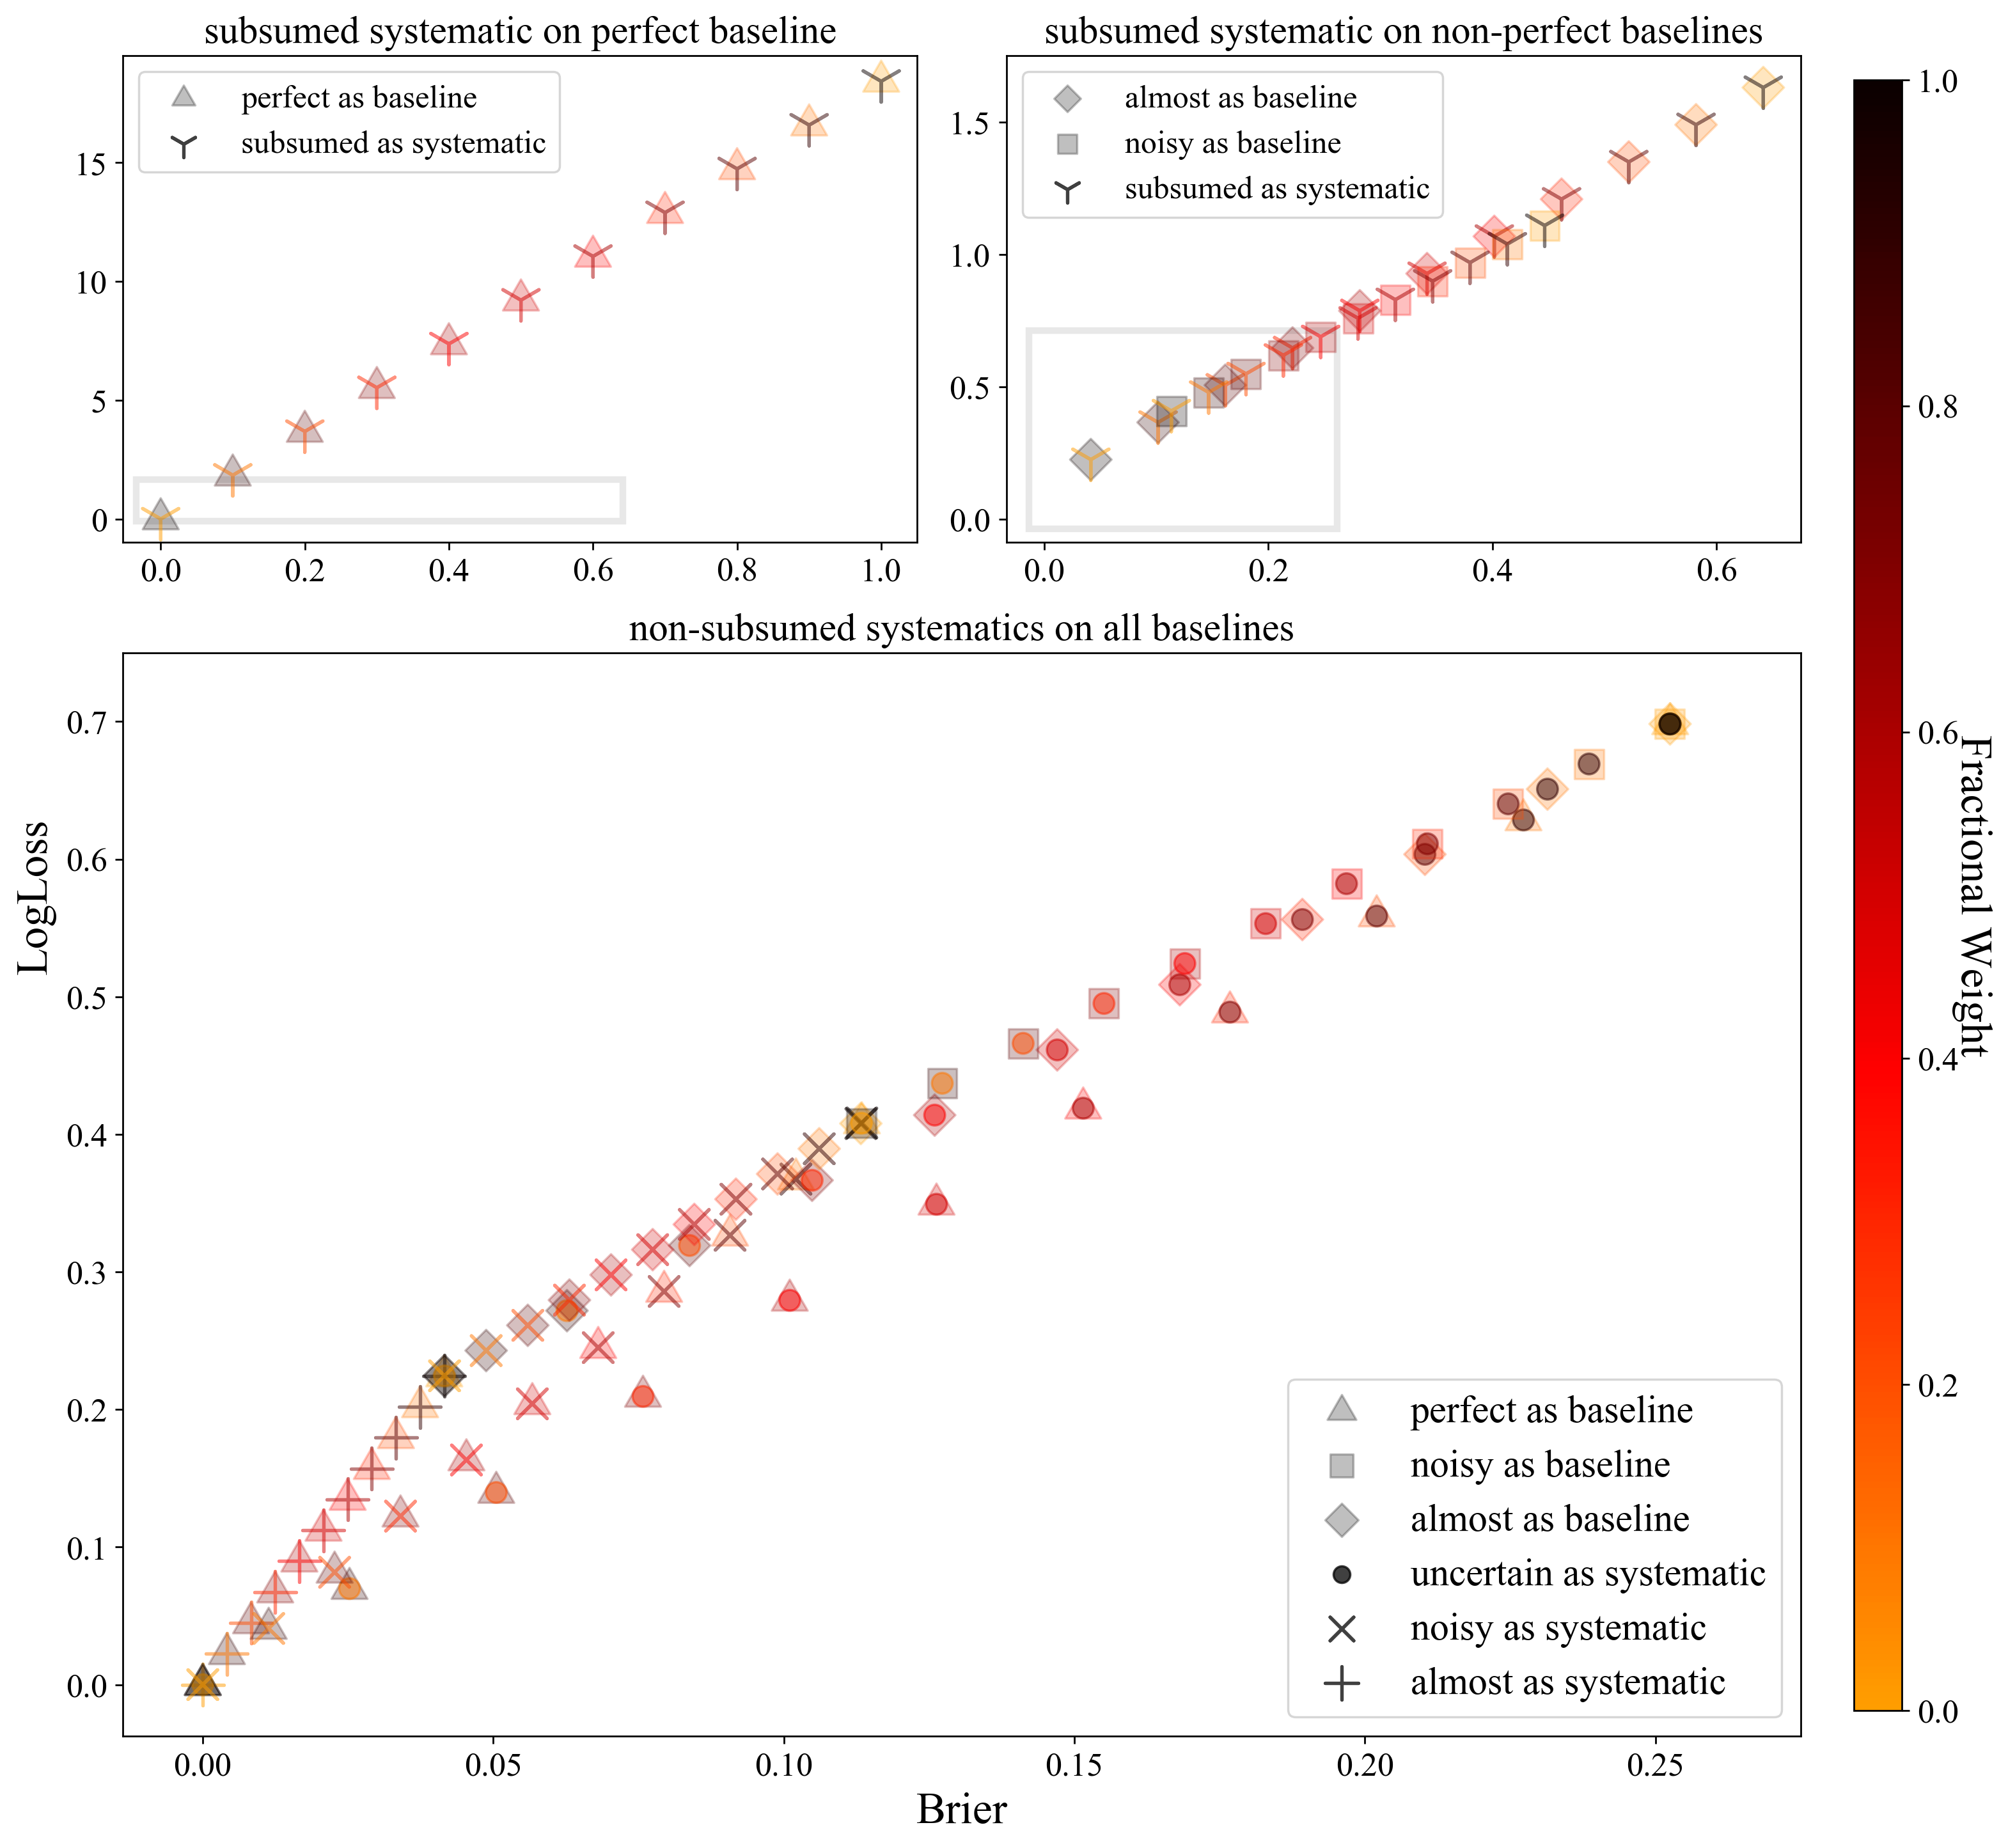
\includegraphics[width=0.99\textwidth]{./fig/multipanel_res.png}
		\caption{Weighted log-loss and Brier scores for baseline classifiers with combinations of systematics.
		Each point represents a classifier with baseline behavior (regular polygon marker) for all but one class with a particular systematic (asterisk markers).
		The color of the systematic effect and baseline behavior markers indicates the weight on the class affected by the systematic and the integrated weight evenly distributed over other classes with baseline behavior, respectively.
		Both metrics are shown in three regimes of sensitivity: to the subsumed systematic on a perfect baseline is highest, all other baselines with the subsumed systematic, and all other systematics.
		The ranges of Brier score and log-loss values between the panels are in ratios of approximately $10:7:3$ and $100:10:5$, respectively, indicating the log-loss's higher sensitivity to the presence of systematics.
		}
	\end{center}
	\label{fig:all_combined}
\end{figure*}

We demonstrate the behavior of the metrics with classification posteriors derived from conditional probability matrices composed of pairs of the characteristic classifiers of Section~\ref{sec:mockdata} is shown in Figure~\ref{fig:all_combined}.
The systematics introduced to each baselines are those that we intuitively expect to worsen performance;
the uncertain, almost perfect, noisy, and subsuming classifiers are anticipated to worsen an otherwise perfect classifier;
the uncertain, noisy, and subsuming classifiers are anticipated to worsen an otherwise almost perfect classifier;
and the uncertain and subsuming classifiers are anticipated to worsen an otherwise noisy classifier.
In every case, we apply the systematic to one true class, i.e. transforming one row of the baseline conditional probability matrix.
The metrics are evaluated at a number of weights $w$ on the affected class, with the weights on the remaining baseline classes equal to one another at $(1 - w) / (M - 1)$.
The weight values range from $0$ (all weight on the baseline) to $1$ (all weight on the systematic) at intervals of $0.1$.
This variation in weights establishes linear relationships between the log-loss and Brier score metrics for each pair of baseline and systematic.

Figure~\ref{fig:all_combined} confirms that for all weight on the perfect classifier, the values of both metrics vanish to zero.
It is immediately evident that the log-loss has more dynamic range than the Brier score overall, and that the log-loss is acutely sensitive to the subsuming systematic on a baseline of a perfect classifier.
In fact, the log-loss value for a classifier that subsumes a class into one that is classified perfectly should actually be infinite if the classes unaffected by the systematic have no weight.
The finite maximum in our tests is set by the artificial zero point established for numerical stability.
Because the combination of a subsuming classifier with a perfect baseline is so different from all other combinations, we separate the subsuming systematic on all other baselines (lower left panel) from all other systematics (lower right panel) in Figure~\ref{fig:all_combined}.
The lower panels of Figure~\ref{fig:all_combined} show that the dynamic range of the log-loss remains higher even outside the regime where it tends toward infinity.
The extent of the values of both metrics is higher in the lower right panel with the subsuming systematic on various baselines than in the lower left panel with all other systematics.
This shows that both metrics are still more sensitive to the subsuming systematic than any other systematic, confirming that both can appropriately penalize the cruise control effect.

\begin{table}[]
\begin{tabular}{lll}
Classifier characteristic & Brier score & Log-loss\\
\hline
Perfect & 0.0 & 0.0\\
Almost perfect & 0.042 & 0.225\\
Noisy & 0.113 & 0.408\\
Uncertain & 0.253 & 0.699\\
Subsumed from Noisy & 0.447 & 1.109\\
Subsumed from Almost & 0.641 & 1.629\\
Subsumed from Perfect & 1.0 & 18.421\footnote{The entry for the log-loss of a classifier that subsumes a class into one that is otherwise perfectly classified should be infinite but is bounded by the numerical precision of our calculations.}
\end{tabular}
\caption{The value of each metric when the weight is entirely on the class(es) with the indicated characteristic.}
\label{tab:extents}
\end{table}

When all weight is on the class affected by a systematic, there is a characteristic limit for each metric's values, shown in Table~\ref{tab:extents}.
Because a subsumed class takes the conditional probability vector of the subsuming class, the metric values depend on what systematics may be affecting the subsuming class as well.
Based on Table~\ref{tab:extents}, both metrics would agree on the ranking of these classifiers, though this agreement is not in general guaranteed.
Furthermore, this invariant ranking is consistent with our intuition about the severity of anticipated faults of classifiers.

\begin{table}[]
\begin{tabular}{l|llll}
	& Systematics & & &\\
Baselines & Subsumed & Uncertain & Noisy & Almost\\
\hline
Perfect & 18.421 & 2.763 & 3.601 & 5.387\\
Almost perfect & 2.343 & 2.246 & 2.556 & \\
Noisy & 2.102 & 2.085 & &
\end{tabular}
\caption{The slopes for each baseline-plus-systematic pair in the space of log-loss  versus Brier score.
A higher slope corresponds to increased sensitivity of the log-loss.}
\label{tab:slopes}
\end{table}

The relative sensitivity ratios of the log-loss to the Brier score are the slopes in the trends of Figure~\ref{fig:all_combined} and are given in Table~\ref{tab:slopes}.
The log-loss always has higher sensitivity than the Brier score, particularly to the difference between the perfect classifier and any lesser classifier.
A possible implication of this behavior is that the log-loss may have an enhanced ability to distinguish between multiple high-performing classifiers that might not have meaningfully different metric values under the Brier score.
In a sense, it means that the log-loss is more susceptible to the tunnel vision classifier, with a significant response to any move toward perfection.
% Heavily unequal weighting can incentivize tunnel vision classification.
% However, the slope is higher for the almost perfect systematic than the noisy systematic, and higher for the noisy systematic than the uncertain systematic; this means that a tunnel vision classifier is deprived of the metric's favor more if it neglects other classes than if it already does fairly well for them, a case in which we would not call it much of a systematic.

% \aim{Still reworking past here.}
% Consider a weighting of $\sim0.8$ for a class affected by tunnel vision, leaving $\sim0.2$ to be shared evenly among all other classes uniformly affected by the other systematics.
% Qualitatively, we would say that a classifier that is almost perfect for other classes is superior to one that is noisy, and a classifier that is noisy for other classes is still superior to one that is uniform; furthermore, the subsuming classifier is even more harshly penalized in this situation than the uncertain classifier, meaning both metrics are  consistent with our basic tests of intuition in this case.
% However, this observation also indicates that the tunnel vision systematic is difficult to penalize, and that if the affected class is given a large weight, it can easily dominate the metric.
% If all classes are of scientific importance, heavily unequal weighting can incentivize tunnel vision classification.

% We introduced weighting of per-class metrics to discourage `tunnel vision' and `cruise control' classifiers that can ignore classes other than the most common and nonetheless perform well by a metric.
% Figure~\ref{fig:popweight} shows the impact of weighting the per-class metrics by the number of objects in the class as each is affected by one of the systematics and the other classes are held at the more realistic almost perfect performance.
% The points show different classification schemes, and all points are coloured by the change in the weighting, dependent on the size of the population class being classified.
% Conversely, the cruise control classifier and, to a lesser degree the noisy classifier, always has high log-loss and Brier score values regardless of the weight on the affected class.

% \begin{figure}
% 	\begin{center}
% 		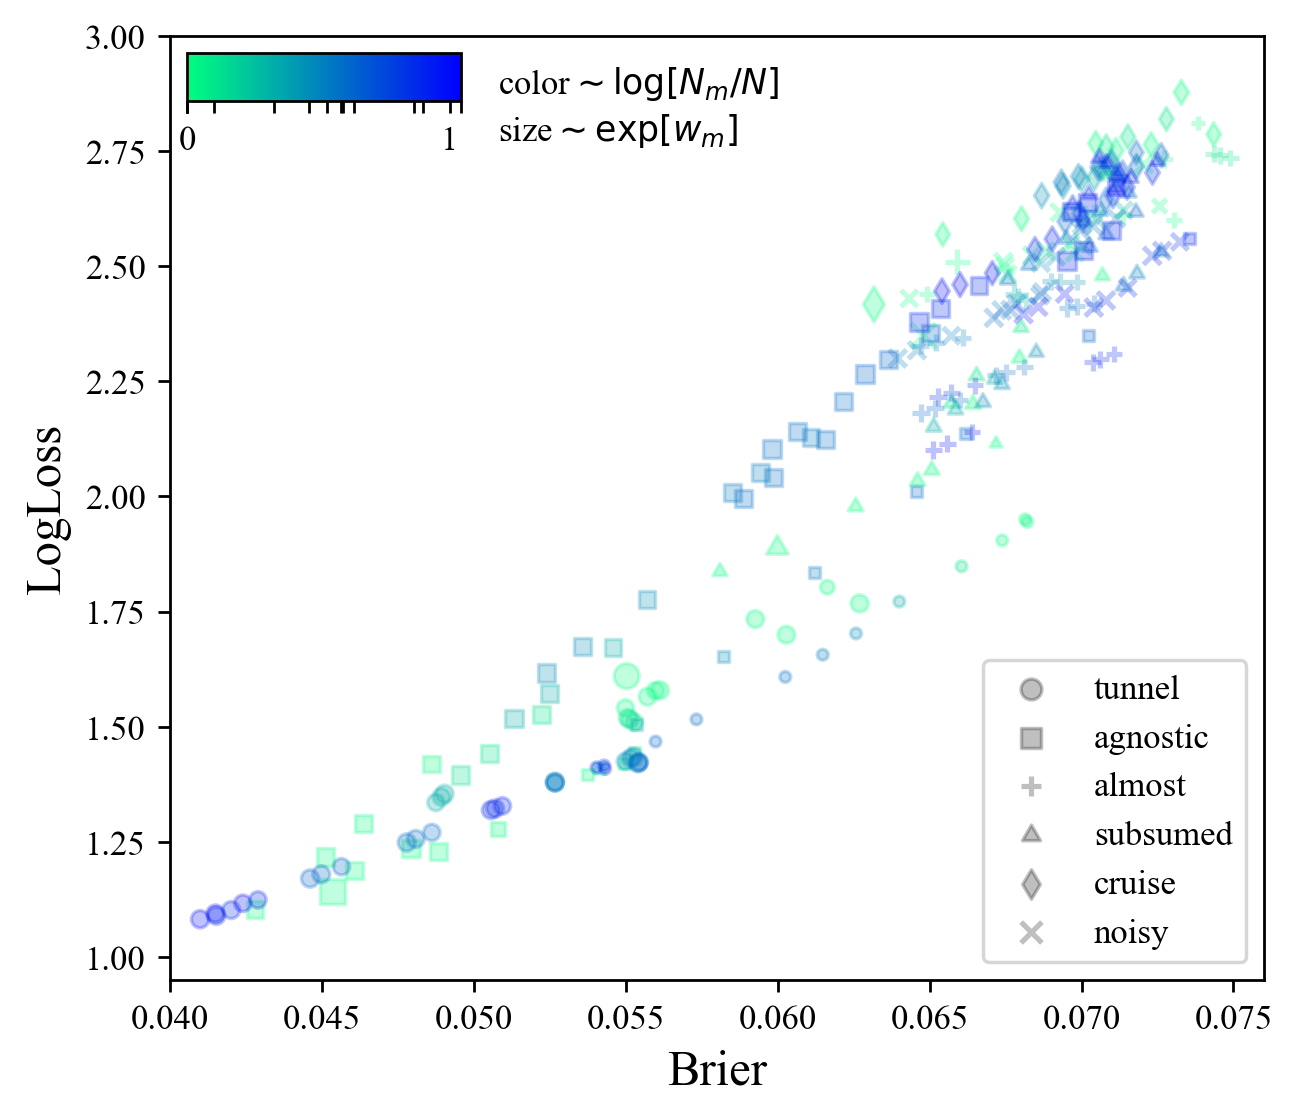
\includegraphics[width=0.5\textwidth]{./fig/all_effects_isolated.png}
% 		\caption{Population-weighted log-loss and Brier scores for classifiers with one class affected by a systematic, as a function of the population of the affected class.
% 		Each point corresponds to an almost perfect classifier that with one class instead affected by a systematic (shape), with log-loss on the $y$ axis and Brier score on the $x$ axis.
% 		The metrics are calculated with a weighting (color and size) proportional to the log of its weight in a weighted average following Equation~\ref{eq:weightavg}.
% 		}
% 	\end{center}
% 	\label{fig:popweight}
% \end{figure}

% The tunnel vision classifier has a consistently low value under the Brier score and log-loss metric (bottom left corner of the plot), only increasing its Brier score once the weighting drops (less blue).
% In this view, the Brier score appears to be more susceptible to tunnel vision than the log-loss, demonstrating a more significant decrease as the size of the affected class increases, but both metrics have concerning behavior in this regard.
% This finding suggests that weighting alone may not be sufficient to counter the influence of this effect, and indicates a need for another balancing mechanism, such as requiring a threshold metric value on all classes.
% When considering a method of converting from one of these metrics to a finall `winner' of the classification challenge, care must be taken to ensure that all approaches do reasonably well at classifying more than one object.
% This thresholding procedure is discussed in the text

% \textbf{Ashish to reaplce/add more here?}
%\aim{Preliminary results indicate weighting will be very important for preventing the tunnel vision classifier from winning. It may be necessary to a priori anticipate which classes will have to be most strongly protected from this systematic via upweighting them.}

%\begin{figure}
%	\begin{center}
%		% 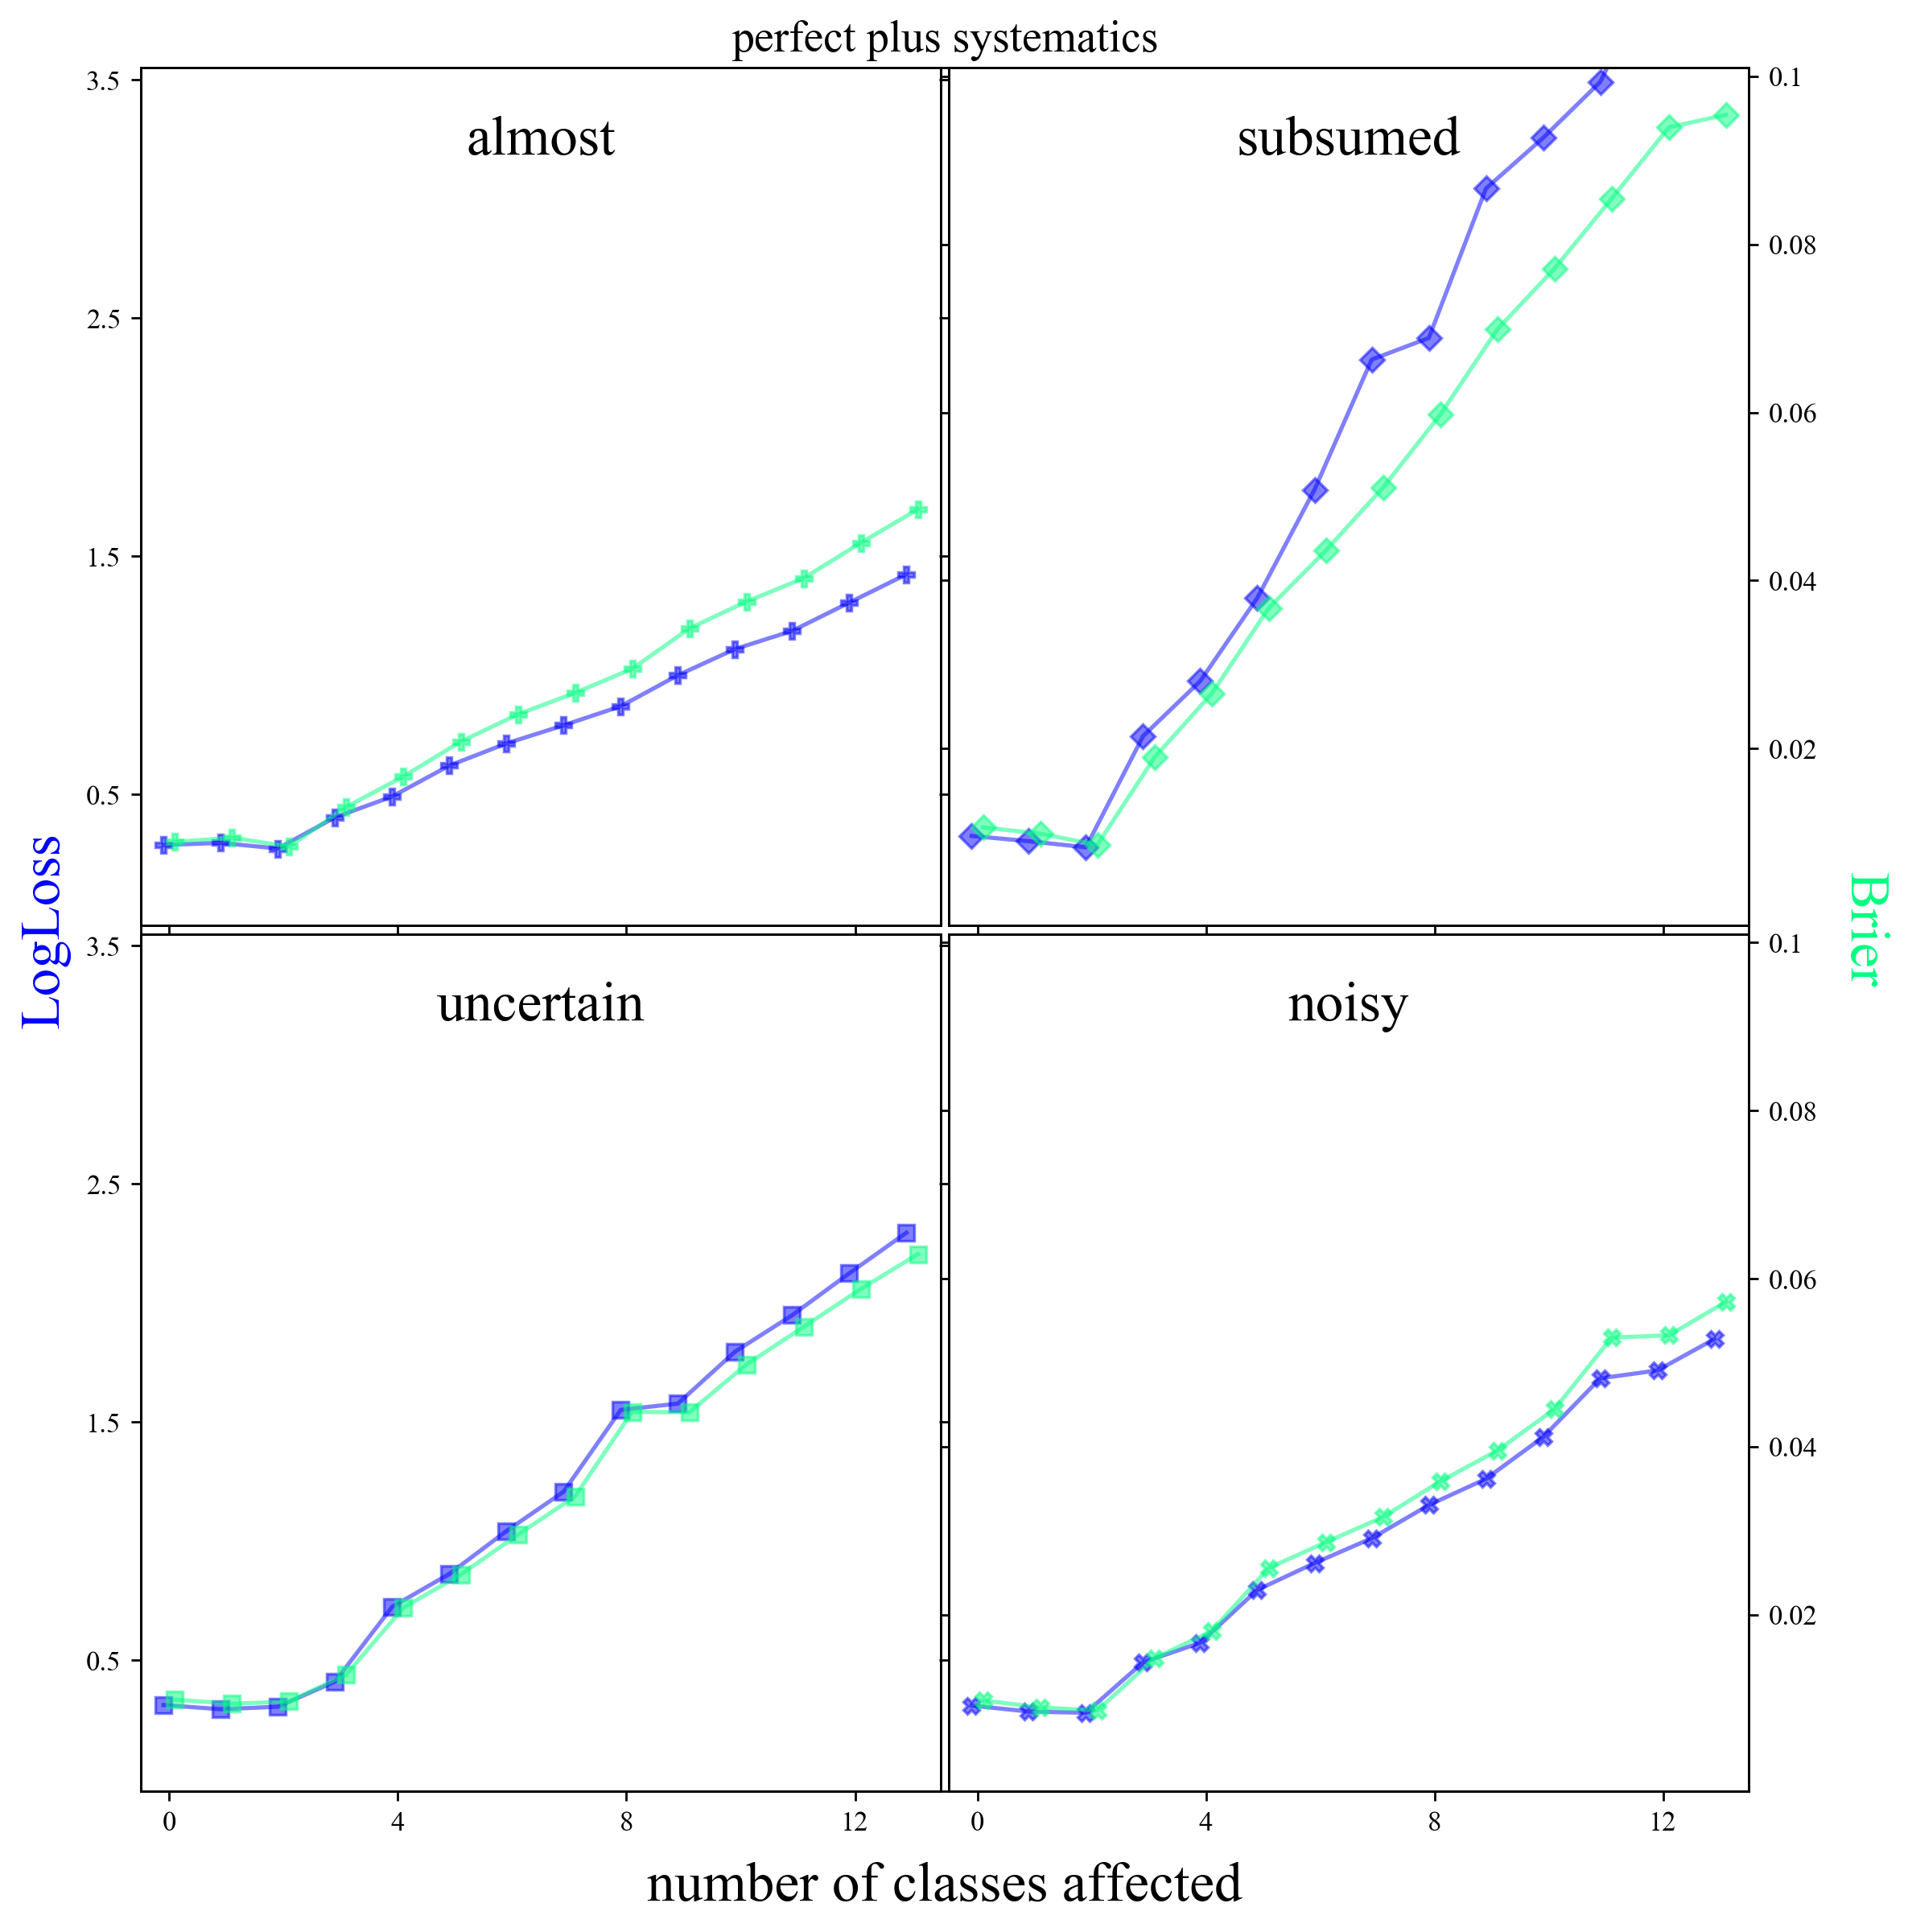
\includegraphics[width=0.5\textwidth]{./fig/systematics_onlyperfect.png}
%		\caption{\aim{After much iteration on how best to present these tests, a figure similar to Figure~\ref{fig:cruise} but for the tunnel vision classifier (heading) on different baseline classifications (panels) as a function of weight on the affected class (rather than number of classes) is under construction.}}
%		\label{fig:tunnel}
%	\end{center}
%\end{figure}

\subsection{Representative classifications}
\label{sec:realresults}

\begin{centering}
\begin{table*}[]
\begin{tabular}{lllllll}%ll}
Rank $R$ & $R_\mathrm{FoM}$ & (FoM) & %$R_\mathrm{AUC}$ & (AUC) &
$R_\mathrm{LogLoss}$ & (Logloss) & $R_\mathrm{Brier}$ & (Brier) \\
\hline
1  & TBRF & 0.635  %& TBRF & 0.982
& TBRF & 0.0907 & TBRF & 0.0486 \\
2  & WBRF & 0.591  %& WBRF & 0.978
& TSVM & 0.113  & TSVM & 0.0583 \\
3  & TSVM & 0.514  %& TSVM & 0.969
& TNN  & 0.125  & TNN  & 0.0650 \\
4  & WSVM & 0.499  %& WSVM & 0.968
& WSVM & 0.1316 & WBRF & 0.0689 \\
5  & TNN  & 0.496  %& TNN  & 0.954
& WBRF & 0.1321 & WSVM & 0.0730 \\
6  & WNN  & 0.480  %& WNN  & 0.946
& TKNN & 0.146  & WNN  & 0.0750 \\
7  & TKNN & 0.384  %& TKNN & 0.942
& WNN  & 0.152  & TKNN & 0.0787 \\
8  & TNB  & 0.340  %& WKNN & 0.894
& WKNN & 0.228  & TNB  & 0.1050 \\
9  & WKNN & 0.114  %& TNB  & 0.879
& TNB  & 0.251  & WKNN & 0.1320 \\
10 & WNB  & 0.0365 %& WNB  & 0.850
& WNB  & 0.443  & WNB  & 0.1780 \\
\end{tabular}
	\caption{The values of three metrics for each of ten \snmachine\ classifiers with equal weight per object.
	The metrics broadly agree on the ranking of the classifiers, confirming consistency between a conventional metric of classification performance and the metrics of probabilistic classifications presented here.}
	\label{tab:snmachineresults}
\end{table*}
\end{centering}

We present in Table~\ref{tab:snmachineresults} the values of all metrics we considered, under equal weight per object, for classification probabilities derived from running the algorithms of \citet{lochner_photometric_2016} on the \snphotcc\ data of Section~\ref{sec:realdata}.
Table~\ref{tab:snmachineresults} also contains the ranking of classifier performance under each metric.

The FOM of Section~\ref{sec:science} differs more from the Brier and log-loss metrics than they do from one another, yet all three metrics are in agreement over the winners and losers, indicating that both of the potential \plasticc\ metrics are roughly consistent with our intuition about what makes a good classifier.
However, this agreement is not universal; the classifiers do not agree with one another on the entire ranking and could thus potentially disagree about the winner .


%\textbf{Current plan is that we compute the SNPhotCC metric for Michelle's contributions and also turn the binary classifications into probabilities - Renee will flesh this out}
%\aim{We are still iterating on the most informative tests to conduct on the \snphotcc\ data.
%I would like to have the confusion matrices from a real classification challenge (\snphotcc\ or Ashish Mahabal's) and test different weightings of our metrics on mock classification probabilities derived from those confusion matrices to check whether we choose the same ``winner,'' but the arrangements have not yet been finalized.
%The ``pipeline,'' however, is complete and ready to run as soon as the test conditions are agreed upon.}


\section{Discussion}
\label{sec:discussion}

The goal of this work is to identify the metric most suited to \plasticc, which seeks classification posteriors of complete light curves similar to those anticipated from \lsst, with an emphasis on classification over all types, rewarding a ``best in show'' classifier rather than focusing on any one class or scientific application.\footnote{At the conclusion of \plasticc, other metrics specific to scientific uses of one or more particular classes will be used to identify ``best in class'' classification procedures that will be useful for more targeted science cases.}
The weighted log-loss is thus the metric most suited to the current \plasticc\ release.

\sout{Future releases of \plasticc\ will focus on different challenges in transient and variable object classification, with metrics appropriate to identifying methodologies that best enable those goals.
We discuss approaches to identifying optimal metrics for these variations, which may be developed further in future work.}
\changes{Transient and variable object classification is crucial for a variety of scientific objectives.
The impact of a shared performance metric on this diversity of goals leads to complex and covariant trade-offs, which thus must be evaluated using multiple metrics.
While a detailed accounting of these possibilities for future releases of \plasticc\ and the selection of appropriate metrics for individual science cases are outside the scope of this first investigation, we discuss below some issues concerning the identification of metrics for a few example science cases.}

\subsection{\sout{Early classification} \changes{Ongoing transient follow-up}}
\label{sec:early}

Spectroscopic follow-up is only expected of a small fraction of \lsst's detected transients and variable objects due to limited resources for such observations.
In addition to optical spectroscopic follow-up, photometric observations in other wavelength bands (near infrared and x-ray from space; microwave and radio from the ground) \changes{or at different times} will be key to building a physical understanding of the object, particularly as we enter the era of multi-messenger astronomy with the added possibility of optical gravitational wave signatures.
Prompt follow-up observations are highly informative for fitting models to the light curves of familiar source classes and to characterizing anomalous light curves that could indicate never-before-seen classes that have eluded identification due to rarity or faintness.
As such, decisions about follow-up resource allocation must be made quickly and under the constraint that resources wasted on a misclassification consume the budget remaining for future follow-up attempts.
A future version of \plasticc\ focused on early light curve classification should have a metric that accounts for these limitations and rewards classifiers that perform better even when fewer observations of the lightcurve are available.

We consider the decision of whether to initiate follow-up observations to be binary and deterministic.
However, it is possible to conceive of non-binary decisions about follow-up resources; for example, one could choose between dedicating several hours on a spectroscopic instrument following up on one likely candidate or dedicating an hour each on several less likely candidates.
Here, we will discuss a metric for an early classification challenge to be focused on deterministic classification because the conversion between classification posteriors and decisions is uncharted territory that we do not explore at this time.

Even within the scope of spectroscopic follow-up as a primary motivation for early light curve classification, the goals of model-fitting to known classes and discovery of new classes would likely not share an optimal metric.
The critical question for choosing the most appropriate metric for any specific science goal motivating follow-up observations is to maximize information.
We provide two examples of the kind of information one must maximize via early light curve classification and the qualities of a deterministic metric that might enable it.

\changes{\subsection{Spectroscopic supernova cosmology}}
\label{sec:spec_sncosmo}

Supernova cosmology with spectroscopically confirmed light curves benefits from true positives, which contribute to the constraining power of the analysis by including one more data point;
when the class in which one is interested is as plentiful as SN Ia and our resources limited a priori, we may not be concerned by a high rate of false negatives.
% requires making a decision balancing the improved constraining power of including another SN Ia in the analysis, thereby constraining the cosmological parameters, so only true positives contribute information, and if we had a perfect classifier and standard follow-up spectroscopy resources, there would be a maximum amount of information about the cosmological parameters that could be gained in this way.
% Each false positive uses the same resources but adds no information about the cosmological parameters, and each false negative consumes no follow-up resources and deprives the Hubble diagram of one more data point.
False positives, on the other hand, may not enter the cosmology analysis, but they consume follow-up resources, thereby depriving the endeavor of the constraining power due to a single SN Ia.

A perfect classifier would lead to a maximum amount of information about the cosmological parameters conditioned on the follow-up resource budget.
\sout{For this scientific application, the metric must be chosen to balance the value of the information forgone by a false positive and the value of information forgone by a false negative, and the value placed on these is effectively weighted by the value we as researchers place on follow-up resources.}
\changes{Consider deterministic labels derived from cutoffs in probabilistic classifications for this scientific application; raising the probability cutoff reduces the number of false positives, boosting the cosmological constraining power, but at a cost of increasing the number of false negatives, which represent constraining power forgone.
As this tradeoff is asymmetric, it is insufficient to consider only the true and false positive and negative rates, as the \snphotcc\ FoM does, without propagating their impact on the information gained about the cosmological parameters.}
% \aim{Cite some deterministic metrics relating to TP/FP?}

\changes{\subsection{Anomalous transient and variable detection}}
\label{sec:anom}

\changes{A particularly exciting science case is anomaly detection, the discovery of entirely unknown classes of transient or variable astrophysical sources, or distinguishing some of the rarest types of sources from more abundant types.
Like the case of spectroscopic supernova cosmology discussed above,} anomaly detection also gains information only from true positives, but the cost function is different in that the potential information gain is unbounded when there is no prior information about undiscovered classes.
% \aim{COMMENT RB: not to stay in doc, but I don't understand the prev sentence. I would also object to the recent detection of kilonova as a good example of anomaly detection, I can buy it if I squint very hard
% COMMENT AIM: Agreed, but I couldn't think of a better one at the time of writing.}
\sout{An example would be the recent detection of a kilonova, flagged initially by the detection of gravitational waves from an object.}
\changes{The discovery of pulsars serves as an example of novelty detection enabled by a human classifier \citep{hewish_observation_1968, bell_burnell_measurement_1969}.}

Resource availability for identifying new classes is more flexible, increasing when new predictions or promising preliminary observations attract attention, and decreasing when a discovery is confirmed and the new class is established.
In this way, a false positive does not necessarily consume a resource that could otherwise be dedicated to a true positive, and the potential information gain is sufficiently great that additional resources would likely be allocated to observe the potential object.
% A false negative, on the other hand, represents forgoing an unbounded quantity of information, so minimizing the false negative rate is as important as maximizing the true positive rate.
% For a rare event like a kilonova, a false negative represents an unbounfalse positive does not appreciably reduce the amount of remaining information available to collect, but a false negative represents a large quantity of information forgone.
% Furthermore, r
% In this case, the information forgone by a false negative is significant compared to the information forgone by a false positive.
Thus, a metric \sout{tuned to} \changes{for evaluating} anomaly detection would aim to \changes{\emph{minimize the false negative rate and maximize the true positive rate.}}
% \aim{Cite some deterministic metrics relating to TP/FN?}

% \subsection{Hierarchical classes}
% \label{sec:hierarchical}
%
% \aim{TODO: We would like to at some point add some content on possible ideas for extending metrics to hierarchical classes, namely conditional extensions of log-loss and possible drawbacks of penalization that can be compensated for by weighting, as well as the challenge that could pose for interpretation.}

\subsection{Difficult light curve classification}
\label{sec:difficult}

Photometric light curve classification may be challenging for a number of reasons, including the sparsity and irregularity of observations, the possible classes and how often they occur, and the distances and brightnesses of the sources of the light curves.
These factors may represent limitations on the information content of the light curves, but appropriate classifiers may be able to overcome them to a certain degree.

Though quality cuts can eliminate the most difficult light curves from entering samples used for science applications, such a practice discards information that may be of value under an analysis methodology leveraging the larger number of light curves included in a sample without cuts.
Thus, classification methods that perform well on light curves characterized by lower signal-to-noise ratios are specially important for exploiting the full potential of upcoming surveys like \lsst.

This version of \plasticc\ implements quality cuts to homogenize difficulty to some degree, and notions of classification difficulty may depend on information that will not be available until after the challenge concludes.
While the groundwork for a metric incorporating data quality has been laid by \citet{wu_radio_2018}, we defer to future work an investigation of this possibility.


\section{Conclusion}
\label{sec:conclusion}

As part of the preparation for \plasticc\, we investigated the properties of metrics suitable for a time-series classification, concentrating on how to reward classifications that performed well across classes, rather than requiring good performance on only one or two classes. In particular we compared the Brier score and the log-loss metrics, and show that that while both metrics could be appropriate metrics for the challenge, the log-loss is slightly more sensitive to systematic affects than the Brier score.

%We have presented an investigative approach to selecting an appropriate metric of the performance of classification techniques producing class posterior probabilities in the context of \plasticc.
%We conclude that the Brier score and log-loss metrics could both be appropriate metrics for \plasticc\ on the basis of their responses to the most concerning systematics anticipated of competing classifiers.
% 
Even though the Brier score and log-loss metrics take values consistent with one another, they are structurally and conceptually different, with wholly different interpretations.
The Brier score is a sum of square differences between probabilities, is harder to map onto a physical interpretation; the explicit penalty term is an attractive feature. The log-loss on the other hand is readily interpretable, meaning the metric itself might serve as a useful way to evaluate different proposed \lsst\ cadences.
 
%to be propagated through forecasting of the constraining power of \lsst\ data.

We perform a weighted averaging between classes to prevent domination by a classifier that focuses exclusively on the most prevalent class, thereby failing to meet \plasticc's diverse goals.  We choose the weighted log-loss for the overall \plasticc\ metric because it is both sensitive to our concerning systematics, and because it is more easily interpretable, with weights to be chosen on the basis of scientific merit (to reward classifications of particular objects). Care must be taken to ensure that the weights between classes are not so severe that they reward classifying all objects as the one particular object of interested.

We note that in order to map on to the Kaggle evaluation platform, a metric weighted only by class was used for the general challenge, while a log-loss with more complicated weighting procedure will be used for the science competition (which will continue for an additional month after the main Kaggle release).

We hope that by investigating metric performance across a range of systematic effects and for a range of weights, we have highlighted both the robustness of the log-loss metric, but also highlighted potential pitfalls of this (and other) metrics.

%We conclude by encouraging the astronomical community to continue to pursue open challenges but to think carefully about the relationship between the goals of a challenge and the global performance metric, as we have done for \plasticc, to ensure that efforts are best directed to achieve the challenge objectives.


% ----------------------------------------------------------------------

\subsection*{Acknowledgments}

%%% Here is where you should add your specific acknowledgments, remembering that some standard thanks will be added via the \code{desc-tex/ack/*.tex} and \code{contributions.tex} files.

%This paper has undergone internal review in the LSST Dark Energy Science Collaboration. % REQUIRED if true

Author contributions are listed below. \\
A.I.~Malz: conceptualization, data curation, formal analysis, investigation, methodology, project administration, software, supervision, validation, visualization, writing - original draft \\
R.~Hlozek: data curation, formal analysis, funding acquisition, investigation, project administration, software, supervision, validation, visualization, writing - original draft \\
T.~Alam: investigation, software, validation \\
A.~Bahmanyar: formal analysis, investigation, methodology, software, writing - original draft \\
R.~Biswas: conceptualization, methodology, software \\
E.E.O.~Ishida: conceptualization, project administration, supervision \\
G.~Narayan: data curation, formal analysis \\
D.~Jones: software \\
A.~Mahabal: data curation, software \\
R.~Martinez-Galarza: data curation, software, visualization \\
C.~Setzer: software \\
 % Standard papers only: author contribution statements. For examples, see http://blogs.nature.com/nautilus/2007/11/post_12.html

% This work used TBD kindly provided by Not-A-DESC Member and benefitted from comments by Another Non-DESC person.

% Standard papers only: A.B.C. acknowledges support from grant 1234 from ...
The authors would like to thank Melissa Graham, Weikang Lin, and Chad Schafer for serving as the LSST-DESC publication review committee.
The authors further wish to thank Kaisey Mandel, Tom Loredo, Rick Kessler, and Lluis Galbany for helpful feedback provided in the preparation of this paper.

AIM is advised by David W. Hogg and was supported by National Science Foundation grant AST-1517237.
TA is supported in part by STFC.
RB and CS are supported by the Swedish Research Council (VR) through the Oskar Klein Centre. Their work was further supported by the research environment grant ``Gravitational Radiation and Electromagnetic Astrophysical Transients (GREAT)'' funded by the Swedish Research council (VR) under Dnr 2016-06012.

Canadian co-authors acknowledge support from the Natural Sciences and Engineering Research Council of Canada.
The Dunlap Institute is funded through an endowment established by the David Dunlap family and the University of Toronto.
The authors at the University of Toronto acknowledge that the land on which the University of Toronto is built is the traditional territory of the Haudenosaunee, and most recently, the territory of the Mississaugas of the New Credit First Nation. They are grateful to have the opportunity to work in the community, on this territory.

We acknowledge the University of Chicago Research Computing Center for support of this work.
This research used resources of the National Energy Research Scientific Computing Center (NERSC), a U.S. Department of Energy Office of Science User Facility operated under Contract No. DE-AC02-05CH11231.

The DESC acknowledges ongoing support from the Institut National de Physique Nucl\'eaire et de Physique des Particules in France; the Science \& Technology Facilities Council in the United Kingdom; and the Department of Energy, the National Science Foundation, and the LSST Corporation in the United States.  DESC uses resources of the IN2P3 Computing Center (CC-IN2P3--Lyon/Villeurbanne - France) funded by the Centre National de la Recherche Scientifique; the National Energy Research Scientific Computing Center, a DOE Office of Science User Facility supported by the Office of Science of the U.S.\ Department of Energy under Contract No.\ DE-AC02-05CH11231; STFC DiRAC HPC Facilities, funded by UK BIS National E-infrastructure capital grants; and the UK particle physics grid, supported by the GridPP Collaboration.  This work was performed in part under DOE Contract DE-AC02-76SF00515.
 % also available: key standard_short

% This work used some telescope which is operated/funded by some agency or consortium or foundation ...

% The DESC acknowledges ongoing support from the Institut National de Physique Nucleaire et de Physique des Particules in France; the Science \& Technology Facilities Council in the United Kingdom; and the Department of Energy, the National Science Foundation, and the LSST Corporation in the United States.
%
% DESC uses resources of the IN2P3 Computing Center (CC-IN2P3--Lyon/Villeurbanne - France) funded by the Centre National de la Recherche Scientifique; the National Energy Research Scientific Computing Center, a DOE Office of Science User Facility supported by the Office of Science of the U.S. Department of Energy under Contract No. DE-AC02-05CH11231; STFC DiRAC HPC Facilities, funded by UK BIS National E-infrastructure capital grants; and the UK particle physics grid, supported by the GridPP Collaboration.
%
% This work was performed in part under DOE Contract DE-AC02-76SF00515.

% We acknowledge the use of An-External-Tool-like-NED-or-ADS.

%{\it Facilities:} \facility{LSST}

% Include both collaboration papers and external citations:
\bibliography{main,lsstdesc}

\end{document}

% ======================================================================
